\chapter{Complex Analysis}
A simple algebraic equation like $x^{2}=-1$ may not have a real solution. Introducing complex numbers validates the existence of 'root' for every polynomial with a positive degree . Which then proves the fundamental theorem of algebra. The idea of complex numbers are widely used in Physics and Mathematics.
\begin{definition}
	A number of the form {${x+i y}$} , where $x$ and $y$ are real numbers and $i=\sqrt{(-1)},$ is called a complex number.
\end{definition}
	\textbf{\large Real Part\ \hspace{1.08cm}:} $x$ is called the real part of the complex number,  $x+i y$ and is written as,\ ${{R(x+i y)}}$.\\\\ 
	\textbf{\large Imaginary Part\ :} $y$ is called the imaginary part of the complex number and is written as,\ ${I(x+i y)}$.
	\section{Representation of a Complex number}
The point whose cartesian coordinates are $(x, y)$ uniquely
represents the complex number, {${z=x+i y}$} on the complex plane $z$. The diagram in which this representation is carried out is called the Argand's diagram. It's shown in the figure \ref{Argand Diagram}.  Since $x$ is the real part of $z$ we call the $x$ -axis the real axis. Likewise, the $y$ -axis is the imaginary axis.

		\begin{figure}[H]
				\begin{center}
			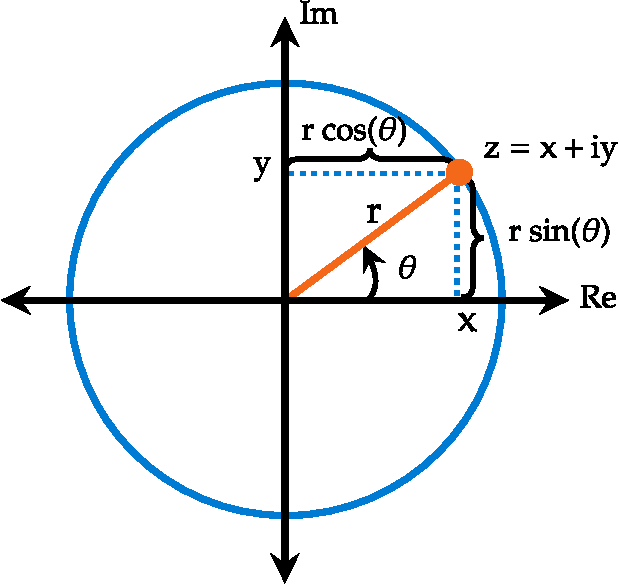
\includegraphics[width=0.30\textwidth]{cn1}
				\end{center}
			\caption{Argand Diagram}
			\label{Argand Diagram}
	    \end{figure}
    In terms of the polar coordinates  , we have
    \begin{align}
    x&=r \cos \theta, \quad y=r \sin \theta\\
    z&=x+\text { iy }=re^{i\theta} \notag \\&=r(\cos \theta+i \sin \theta)
    \label{Euler's equation}
    \end{align}
    Then, the  equation \ref{Euler's equation} is known as, Euler's formula
    \begin{figure}[H]
    	\begin{minipage}{0.40\textwidth}
    		\begin{center}
    		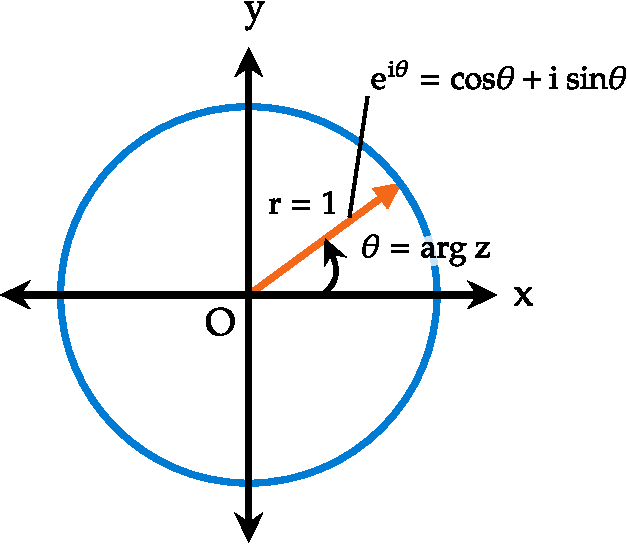
\includegraphics[width=0.70\textwidth]{cn2}
    	\end{center}
    	\end{minipage}\hfil
    	\begin{minipage}{0.40\textwidth}
    	\begin{center}
    		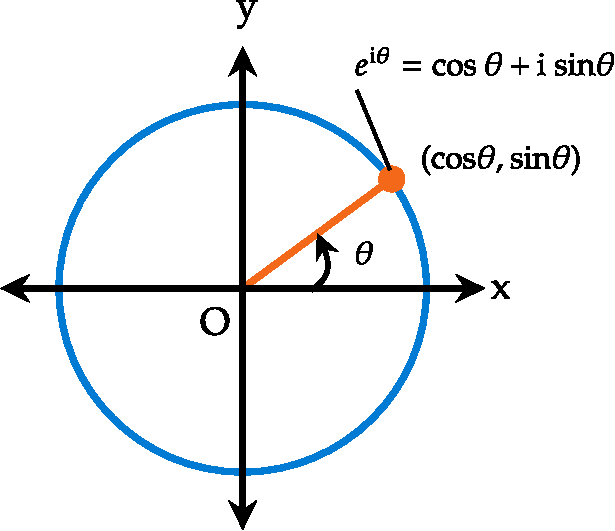
\includegraphics[width=0.70\textwidth]{cn3}
    	\end{center}
    \end{minipage}
    
    \caption{Polar representation}
    \end{figure}
   \subsection{Absolute Value}
    We define the absolute value of a complex number $x+i y$ to be the length ${r}$ of the vector from the origin to $P(x, y)$. 
    $$
    r=|x+i y|=\sqrt{x^{2}+y^{2}}
    $$
    \\\textbf{Properties:}
    \begin{itemize}
    	\item $\left|z_{1}+z_{2}\right| \leq\left|z_{1}\right|+\left|z_{2}\right|$
    	\item $\left|z_{1}-z_{2}\right| \geq\left|z_{1}\right|-\left|z_{2}\right|$
    	\item $\left|z_{1} z_{2}\right|=\left|z_{1}\right|\left|z_{2}\right|$
    	\item $\left|\frac{z_{1}}{z_{2}}\right|=\frac{\left|z_{1}\right|}{\left|z_{2}\right|}$
    \end{itemize}
    \subsection{Argument of }
    The polar angle $\theta$ is called the {argument} of $z$ and it is written as, $${\theta=\arg z }$$ Any integer multiple of $2 \pi$ may be added to $\theta$ to produce another appropriate  angle.\\From the figure \ref{Argand Diagram},
    $${\theta=\arg z }=\tan ^{-1}\left(\frac{y}{x}\right)$$
    \\\textbf{Properties:}
    \begin{itemize}
    	\item $\operatorname{Arg}\left(z_{1}  z_{2} \cdot z_{3} \ldots \ldots z_{n}\right)=\operatorname{Arg} \left(z_{1}\right)+\operatorname{Arg}  \left(z_{2}\right)+\operatorname{Arg}  \left(z_{3}\right)+\ldots \ldots . .+\operatorname{Arg}\left(z_{n}\right)$
    	\item $\operatorname{Arg}\left(\frac{z_{1}}{z_{2}}\right)=\operatorname{Arg}\left(z_{1}\right)-\operatorname{Arg}\left(z_{2}\right)$
    \end{itemize}
\begin{exercise}
	Find the modulus and principal argument of the complex number
	$\frac{1+2 i}{1-(1-i)^{2}}$
\end{exercise}
\begin{answer}
	\begin{align*}
	\frac{1+2 i}{1-(1-i)^{2}}&=\frac{1+2 i}{1-(1-1-2 i)}=\frac{1+2 i}{1+2 i}\\&=1=1+0 i \\
	\therefore \quad\left|\frac{1+2 i}{1-(1-i)^{2}}\right|&=|1+0 i|=\sqrt{1^{2}}=1\\
	\text{Principal argument of}\ \frac{1+2 i}{1-(1-i)^{2}}&= \text{Principal argument of} \quad \left( 1+0 i\right) \\
	\tan ^{-1} \frac{0}{1}&=\tan ^{-1} 0\\&=0^{\circ}
	\end{align*}
\end{answer}
     \subsection{Conjugate of a Complex number}
	The conjugate of a complex number $z$ is represented by, $${\bar{z}=x-i y}$$
	\begin{note}\newline 
	$ \left. \right. $ \hspace{1.5cm}	
	$\begin{aligned}
		\frac{z + \bar{z}}{2}&=Re\left\lbrace z\right\rbrace \\
		\frac{z - \bar{z}}{2i}&=Im\left\lbrace z\right\rbrace\\
		z \cdot \bar{z}&=|z|^{2}
		\end{aligned}$
	\end{note}
\section{Algebra of Complex numbers}
For two Complex numbers, $a+i b$ and $c+i d $
\subsubsection{Equality:}
	\begin{align*}
	a+i b&=c+i d \quad
	\end{align*}
	Two complex numbers $(a, b)$
 and $(c, d)$ are equal if and only $a=c$ and $b=d$.
 \subsubsection{Addition:} 
 \begin{align*}
 (a+i b)+(c+i d) \quad&=(a+c)+i(b+d) \quad
 \end{align*}
 \subsubsection{Multiplication:} \begin{align*}
 (a+i b)(c+i d) &=(a c-b d)+i(a d+b c) \\
 c(a+i b)&=a c+i(b c)
 \end{align*}
 \textbf{Polar form:} 
 \begin{align*} 
 \text{Let,} \quad z_{1}&=r_{1}\left(\cos \theta_{1}+i \sin \theta_{1}\right) \quad \text{and}\quad z_{2}=r_{2}\left(\cos \theta_{2}+i \sin \theta_{2}\right)\\
 z_{1} . z_{2} &=r_{1} r_{2}\left(\cos \theta_{1}+i \sin \theta_{1}\right)\left(\cos \theta_{2}+i \sin \theta_{2}\right) \\ &=r_{1} r_{2}\left[\cos \theta_{1} \cos \theta_{2}-\sin \theta_{1} \sin \theta_{2}+i\left(\sin \theta_{1} \cos \theta_{2}+\cos \theta_{1} \sin \theta_{2}\right)\right] \\ &=r_{1} r_{1}\left[\cos \left(\theta_{1}+\theta_{2}\right)+i \sin \left(\theta_{1}+\theta_{2}\right)\right], \end{align*}
 
 \subsubsection{Division:}\begin{align*}
 \frac{c+i d}{a+i b}&=\frac{(c+i d)(a-i b)}{(a+i b)(a-i b)}\\&=\frac{(a c+b d)+i(a d-b c)}{a^{2}+b^{2}}\\
 \text{Where,}\quad x&=\frac{a c+b d}{a^{2}+b^{2}},\quad \text{and} \quad y=\frac{a d-b c}{a^{2}+b^{2}}
 \end{align*}
 
\section{Important Identities}
\subsection{Circular functions of Complex numbers}

\begin{align*}
	\bullet\quad\sin \theta=\frac{e^{i \theta}-e^{-i \theta}}{2 i}\quad\bullet&\quad\cos \theta=\frac{e^{i \theta}+e^{-i \theta}}{2}\\\\
\bullet\quad\sin z=\frac{e^{i z}-e^{-i z}}{2 i}\quad\bullet&\quad\cos z=\frac{e^{i z}+e^{-i z}}{2}
\end{align*}

\subsection{Hyperbolic functions of Complex numbers}
\begin{alignat*}{2}
&\bullet\quad \sinh x=\frac{e^{x}-e^{-x}}{2}\quad&&\bullet\quad \cosh x=\frac{e^{x}+e^{-x}}{2}\\
&\bullet\quad\tanh x=\frac{e^{x}-e^{-x}}{e^{x}+e^{-x}}\quad&&\bullet \quad {\coth} x=\frac{e^{x}+e^{-x}}{e^{x}-e^{-x}}
\\
&\bullet\quad{\operatorname{sech}} x=\frac{2}{e^{x}+e^{-x}} \quad&&\bullet \quad {\operatorname{cosech}} x=\frac{2}{e^{x}-e^{-x}}\\
&\bullet\quad\cosh x+\sinh x=\frac{e^{x}+e^{-x}}{2}+\frac{e^{x}-e^{-x}}{2}=e^{x} \quad&& \quad
\end{alignat*}
\begin{note}
\textbf{\textbf{Relation between Circular and Hyperbolic functions:}}\\\\
$\begin{array}{ll}\bullet\quad\sin i x=i \sinh x & \bullet\quad \sinh i x=i \sin x \\ \bullet\quad\cos i x=\cosh x & \bullet\quad \cosh i x=\cos x \\ \bullet\quad\tan i x=i \tanh x& \bullet\quad \tanh i x=i \tan x\end{array}$

\end{note}

\begin{theorem}
	\textbf{De Moivre's Theorem:}
	\begin{enumerate}
		\item For any integer $n,$ $(\cos \theta+i \sin \theta)^{n}=\cos n \theta+i \sin n \theta$
		\item 	If $n$ is a fraction, then $(\cos n \theta+i \sin n \theta)$ is one of the values .
	\end{enumerate}
\end{theorem}
\begin{exercise}
  Express $\frac{(\cos \theta+i \sin \theta)^{8}}{(\sin \theta+i \cos \theta)^{4}}$ in the form $(x+i y)$
\end{exercise}
\begin{answer}
	$$
	\begin{aligned}
	\frac{(\cos \theta+i \sin \theta)^{8}}{(\sin \theta+i \cos \theta)^{4}}=&\frac{(\cos \theta+i \sin \theta)^{8}}{(i)^{4}\left(\cos \theta+\frac{1}{i} \sin \theta\right)^{4}} \\
	=& \frac{(\cos \theta+i \sin \theta)^{8}}{(\cos \theta-i \sin \theta)^{4}}=\frac{(\cos \theta+i \sin \theta)^{8}}{[\cos (-\theta)+i \sin (-\theta)]^{4}} \\
	=& \frac{(\cos \theta+i \sin \theta)^{8}}{\left[(\cos \theta+i \sin \theta)^{-1}\right]^{4}}=\frac{(\cos \theta+i \sin \theta)^{8}}{(\cos \theta+i \sin \theta)^{-4}}=(\cos \theta+i \sin \theta)^{12} \\
	=& \cos 12 \theta+i \sin 12 \theta
	\end{aligned}
	$$
\end{answer}
\begin{note}
	Series expansion of different functions
	\begin{align*}
	e^{x}&=1+x+\frac{x^{2}}{2 !}+\frac{x^{3}}{3 !}+\frac{x^{4}}{4 !}+\ldots \\
	\sin x&=x-\frac{x^{3}}{3 !}+\frac{x^{5}}{5 !}-\frac{x^{7}}{7 !}+\ldots \\
	\cos x&=1-\frac{x^{2}}{2 !}+\frac{x^{4}}{4 !}-\frac{x^{6}}{6 !}+\ldots \\
	\tan x&=x+\frac{x^{3}}{3}+\frac{2 x^{5}}{15}+\frac{17 x^{7}}{315}+\frac{62 x^{9}}{2835} +\cdots\\
	\ln (1+x)&=x-\frac{x^{2}}{2}+\frac{x^{3}}{3}-\frac{x^{4}}{4}+\ldots \\
    \tan ^{-1}(x)&=x-\frac{x^{3}}{3}+\frac{x^{5}}{5}-\frac{x^{7}}{7}+\ldots
	\end{align*}
	\end{note}
	\section{Function of a Complex Variable}
	\subsection{Basic Representation}
	\begin{align*}
	W&=f(z)=v(x, y)+i v(x, y)\hspace{4cm}\text{Real part (u)},\left(x^{2}-y^{2}\right)^{2}\\
	f(z)&=z^{2}=(x+i y)^{2}=\left(x^{2}-y^{2}\right)^{2}+i 2 x y\hspace{3cm}\text{Imaginary part (v)}, 2 x y
	\end{align*}
\subsection{Existance of $\lim _{z \rightarrow z_{0}} f(z)$ :}
		The limit will exists only if the limiting value is independent of the path along which $z$ approaches $z_0$
	\begin{exercise}
		Find whether the limit $\lim _{z \rightarrow 0} \frac{z}{|z|}$ exist or not.
	\end{exercise}
	\begin{answer}
		\begin{align*}
		z \rightarrow 0\text{ means }&x \rightarrow 0 \& y \rightarrow 0\\
		\text{	For }\mathrm{z}&=0,\text{ we have to choose a path passing through a origin.}
	\intertext{	Therefore, we have choosen a straight line passing through the origin i.e. $y=m x$}
		\lim _{z \rightarrow 0} \frac{z}{|z|}&=\lim _{\substack{z \rightarrow 0 \\ y \rightarrow 0}} \frac{x+i y}{\sqrt{x^{2}+y^{2}}}=\lim _{x \rightarrow 0} \frac{x+i m x}{\sqrt{x^{2}+m^{2} x^{2}}}=\frac{1+i m}{\sqrt{1+m^{2}}}
		\intertext{Therefore, the limit depends on m i.e. slope of the straight line. Thus, the limiting values is dependent on the path and the limit does not exists.}
		\end{align*}
	\end{answer}
	\begin{exercise}
		Calculate the vahue $\lim _{z \rightarrow \infty} \frac{i z^{3}+i z-1}{(2 z+3 i)(z-i)^{2}}$
	\end{exercise}
	\begin{answer}
		\begin{align*}
		\lim _{z \rightarrow \infty} \frac{i z^{3}+i z-1}{(2 z+3 i)(z-i)^{2}}=\lim _{z \rightarrow \infty} \frac{z^{3}\left(i+\frac{i}{z^{2}}-\frac{1}{z^{3}}\right)}{z\left(2+\frac{3 i}{z}\right) z^{2}\left(1-\frac{i}{z}\right)^{2}}=\frac{i}{2}
		\end{align*}
	\end{answer}
	\subsection{Differentiability of Complex Function}
	\begin{align*}
	\mathrm{f}^{\prime}(\mathrm{z})&=\underset{\delta \mathrm{z} \rightarrow 0}{\mathrm{Lt}} \frac{[\mathrm{f}(\mathrm{z}+\delta \mathrm{z})-\mathrm{f}(\mathrm{z})]}{\delta \mathrm{z}}
\intertext{	The function will be differentiable if limit should exists and it is independent of path along with $\delta z \rightarrow 0$.}
\text{	Ex: }\quad \mathrm{f}(z)&=(4 x+y)+i(4 y-x) \Rightarrow u=(4 x+y)\text{ and }v=(4 y-x)\\
	&\Rightarrow f(z+\delta z)=4(x+\delta x)+(y+\delta y)+i[4(y+\delta y)-(x+\delta x)] \\
	&\Rightarrow f(z+\delta z)-f(z)=4 \delta x+\delta y+i(4 \delta y-\delta x)\\
	&\Rightarrow \frac{f(z+\delta z)-f(z)}{\delta z}=\frac{4 \delta x+\delta y+i(4 \delta y-\delta x)}{\delta z} \Rightarrow \frac{\delta f}{\delta z}=\frac{4 \delta x+\delta y-i \delta x+4 i \delta y}{\delta x+i \delta y}\\
	&\text{Along real axis : }\delta x=\delta z, \delta y=0, \Rightarrow \frac{\delta f}{\delta z}=4-i\\
	&\text{Along imaginary axis : }i \delta y=\delta z, \delta x=0, \Rightarrow \frac{\delta f}{\delta z}=4-i\\
	&\text{Along a line }: y=x, \delta y=\delta x, \delta z=(1+i) \delta x, \Rightarrow \frac{\delta f}{\delta z}=\frac{5 \delta x+3 i \delta x}{(1+i) \delta \dot{x}}=\frac{5+3 i}{1+i}=4-i
		\end{align*}
	\section{Complex Analysis Function}
	A function $f(z)$ is said to be analytic at a point $z=z_{0}$ if it is single valued and has the derivative at every point in some neighhourhood of $z_{0}$. The function $f(z)$ is said to be analytic in a domain $D$ if it is single valued and is differentiable at every point of domain D.
	\subsection{Cauchy Reamann Equations}
	\begin{align*}
	\intertext{	For a function $f(z)=u+i v$ to be analytic at all points in some region ' $\mathrm{R}$ ', the necessary conditions are:}
		\frac{\partial u}{\partial x}&=\frac{\partial v}{\partial y} \text { and } \frac{\partial u}{\partial y}=-\frac{\partial v}{\partial x}\\
		\text{Sufficient Condition: }&\frac{\partial u}{\partial x}, \frac{\partial u}{\partial y}, \frac{\partial v}{\partial x}, \frac{\partial v}{\partial y}\text{ are continuous functions of $x$ and $y$.}\\
		\text{	Derivative of }\mathrm{f}(\mathrm{z}): f^{\prime}(\mathrm{z})&=\frac{\partial u}{\partial x}+i \frac{\partial v}{\partial x}=\frac{\partial v}{\partial y}-i \frac{\partial u}{\partial y}
	\end{align*}
	\begin{exercise}
		Check whether $f(z)=\sin z$ is analytic or not.
	\end{exercise}
	\begin{answer}
		\begin{align*}
		&f(z)=\sin z=\sin (x+i y)=\sin x \cdot \cos (i y)+\cos x \cdot \sin (i y)=\sin x \cdot \cosh y+i \cos x \cdot \sinh y\\
		&\text{Therefore, }u=\sin x \cdot \cosh y\text{ and }v=\cos x.sinhy \\
		&\frac{\partial u}{\partial x}=\cos x \cdot \cosh y ; \frac{\partial u}{\partial y}=\sin x \cdot \sinh y ; \frac{\partial v}{\partial x}=-\sin x \cdot \sinh y ; \frac{\partial v}{\partial y}=\cos x \cdot \cosh y\\
		&\text { So, C-R equation is satisfied, given } \mathrm{f}(\mathrm{z}) \text { is analytic. }
		\end{align*}
	\end{answer}
	\begin{exercise}
		If the real part of a complex analytic function is $u(x, y)=x+\frac{1}{2}\left(x^{2}-y^{2}\right)$, find the corresponding imaginary part.
	\end{exercise}
	\begin{answer}
		\begin{align*}
		\frac{\partial u}{\partial x}=x+1=\frac{\partial v}{\partial y} & \Rightarrow v(x, y)=y+x y+f(x) \\
		\frac{\partial u}{\partial y}=-y=-\frac{\partial v}{\partial x} & \Rightarrow v(x, y)=x y+g(y)\\
	\text{	Therefore, the imaginary }&\text{part will be }v(x, y)=y+x y+C
	\text{	( $C=$ numerical constant )}
		\end{align*}
	\end{answer}
	\begin{exercise}
		Example-7: If $f(x, y)=(1+x+y)(1+x-y)+a\left(x^{2}-y^{2}\right)-1+2 i y(1-x-a x)$ is a complex analytic function then find the value of ' $a$ '.
	\end{exercise}
	\begin{answer}
		\begin{align*}
		u(\mathrm{x}, \mathrm{y})&=(1+x+y)(1+x-y)+a\left(x^{2}-y^{2}\right)-1 \quad \Rightarrow \frac{\partial u}{\partial x}=2 x+2+2 a x \\
		v(x, y)&=2 y(1-x-a x) \quad \Rightarrow \frac{\partial v}{\partial y}=2(1-x-a x)\\
		\text{According to Cauchy  }&\text{ Reamann equation,}\frac{\partial \mathrm{u}}{\partial \mathrm{x}}=\frac{\partial \mathrm{v}}{\partial \mathrm{y}} \Rightarrow 4 \mathrm{x}=-4 \mathrm{ax} \Rightarrow \mathrm{a}=-1
		\end{align*}
	\end{answer}
	\begin{exercise}
		The harmonic conjugate function of $u(x, y)=2 x(1-y)$ corresponding to a complex analytic function $\omega=u(x, y)+i v(x, y)$ is given $v(x, y)=\alpha x^{2}+\beta y+\gamma y^{2}$ (Taking the integration constant to be zero).
		Which of the following statement is true ?
		 \begin{tasks}(2)
			\task[\textbf{a.}]$\alpha-\gamma=\beta$
			\task[\textbf{b.}]$\alpha+\gamma+\beta=0$
			\task[\textbf{c.}]$\alpha+\gamma=\beta$
			\task[\textbf{d.}] $\alpha \gamma \beta=1$.
		\end{tasks}
	\end{exercise}
	\begin{answer}
		\begin{align*}
		u(x, y)&=2 x(1-y) \\
		\Rightarrow \frac{\partial u}{\partial x}&=2(1-y)=\frac{\partial v}{\partial y} \Rightarrow v=2 y-y^{2}+f_{1}(x) \\
		\Rightarrow \frac{\partial u}{\partial y}&=-2 x=-\frac{\partial v}{\partial x} \Rightarrow v=x^{2}+f_{2}(y)
		\end{align*}
			Therefore, the imaginary part of the complex function $v=x^{2}-y^{2}+2 y$ \\Comparing with the question, $\alpha=1, \beta=2, \gamma=-1 \quad \Rightarrow \alpha-\gamma=\beta$
	\end{answer}
	So the correct answer is \textbf{option (a)}
	\subsection{Cauchy Reamann equations in Polar co-ordiantes:}
	\begin{answer}
		\begin{align*}
		\frac{\partial u}{\partial r}&=\frac{1}{r} \frac{\partial v}{\partial \theta} \text { and } \frac{\partial u}{\partial \theta}=-r \frac{\partial v}{\partial r}\\
		\text{Derivative of }f(z): f^{\prime}(\mathrm{z})&=(\cos \theta-i \sin \theta) \frac{\partial f}{\partial r}=-\frac{i}{r}(\cos \theta-i \sin \theta) \frac{\partial f}{\partial \theta}
		\end{align*}
	\end{answer}
	\subsection{Harmonic Function}
	Any function which satisfies the Laplace's equation, is known as harmonic function. If $u+i v$ is an analytic function, then $u, v$ are conjugate harmonic functions i.e.
	$$
	\frac{\partial^{2} u}{\partial x^{2}}+\frac{\partial^{2} u}{\partial y^{2}}=0 \text { and } \frac{\partial^{2} v}{\partial x^{2}}+\frac{\partial^{2} v}{\partial y^{2}}=0
	$$
	\begin{exercise}
		Find the values of $\mathrm{m}, \mathrm{n}$ such that $f(x, y)=x^{2}+m x y+n y^{2}$ is harmonic in nature.
	\end{exercise}
	\begin{answer}
		\begin{align*}
		\text { Since, } \frac{\partial^{2} f}{\partial x^{2}}+\frac{\partial^{2} f}{d y^{2}}=0 \Rightarrow 2 n+2=0 \Rightarrow n=-1 ;^{\prime} m^{\prime} \text { can take any value. }
		\end{align*}
	\end{answer}
	\subsection{Method for Finding Conjugate Function }
		\begin{align*}
		\textbf{Case 1: }f(z)&=u+i v,\text{ and $u$ is known.}\\
		d v&=\frac{\partial v}{\partial x} d x+\frac{\partial v}{\partial y} d y=-\frac{\partial u}{\partial y} d x+\frac{\partial u}{\partial x} d y \Rightarrow v=-\int \frac{\partial u}{\partial y} d x+\int \frac{\partial u}{\partial x} d y\\
		\textbf{Case 2: }f(z)&=u+i v,\text{ and $v$ is known}\\
		d u&=\frac{\partial u}{\partial x} d x+\frac{\partial u}{\partial y} d y=\frac{\partial v}{\partial y} d x-\frac{\partial v}{\partial x} d y \Rightarrow u=\int \frac{\partial v}{\partial y} d x-\int \frac{\partial v}{\partial x} d y
		\end{align*}
	\begin{exercise}
		 Find the imaginary part of the complex analytic function whose real part is $u(x, y)=x^{3}-3 x y^{2}+3 x^{2}-3 y^{2}+1$
	\end{exercise}
	\begin{answer}
		\begin{align*}
		&\frac{\partial u}{\partial x}=3 x^{2}-3 y^{2}+6 x=\frac{\partial v}{\partial y} \Rightarrow v=3 x^{2} y-y^{3}+6 x y+f_{1}(x) \\
		&\frac{\partial u}{\partial y}=-6 x y-6 y=-\frac{\partial v}{\partial x} \Rightarrow v=3 x^{2} y+6 x y+f_{2}(y) \\
		&v(x, y)=3 x^{2} y-y^{3}+6 x y+C
		\end{align*}
	\end{answer}
	\subsection{Milne-Thomson Method : (To find Analytic function if either ' $u$ ' or ' $v$ ' is given)}
	\begin{align*}
\textbf{	Case 1:}&\text{ When 'u' is given,}\\
	&\text{(1) Find }\frac{\partial u}{\partial x}=\phi_{1}(x, y) \text{and }\frac{\partial u}{\partial y}=\phi_{2}(x, y)\\
	&\text{(2) Replace }\text{$x$ by $z$ and $y$ by 0 in $\phi_{1}(x, y)$ and $\phi_{2}(x, y)$ to get $\phi_{1}(z, 0)$ and $\phi_{2}(z, 0)$.}\\
	&\text{(3) Find }f(z)=\int\left\{\phi_{1}(z, 0)-i \phi_{2}(z, 0)\right\} d z+c\\
\textbf{	Case 2: }&\text{When ' $v$ ' is given,}\\
&\text{	(1) Find }\frac{\partial v}{\partial x}=\psi_{2}(x, y)\text{ and }\frac{\partial v}{\partial y}=\psi_{1}(x, y)\\
&\text{(2) Replace }\text{$x$ by $z$ and $y$ by 0 in $\psi_{1}(x, y)$ and $\psi_{2}(x, y)$ to get $\psi_{1}(z, 0)$ and $\psi_{1}(z, 0)$.}\\
&\text{(3) Find }f(z)=\int\left\{\psi_{1}(z, 0)+i \psi_{2}(z, 0)\right\} d z+c
	\end{align*}
	\begin{exercise}
		Find the analytical function whose imaginary part is $v(x, y)=e^{x}(x \cos y-y \sin y)$
	\end{exercise}
	\begin{answer}
		\begin{align*}
		\frac{\partial v}{\partial x}=e^{x}(x \cos y-y \sin y)+e^{x} \cos y=\Psi_{2}(x, y) \quad& \Rightarrow \frac{\partial v}{\partial y}=-e^{x} x \sin y-e^{x}(\sin y+y \cos y)=\Psi_{1}(x, y) \\
		\Psi_{1}(z, 0)=0 \text { and } \Psi_{1}(z, 0)=e^{z} z+e^{z} \quad& \Rightarrow f(z)=\int 0+i\left[e^{z} z+e^{z}\right] d z=i z e^{z}+C
		\end{align*}
	\end{answer}
	\begin{exercise}
		 If the real part of a complex analytic function $\mathrm{f}(\mathrm{z})$ is given as, $u(x, y)=e^{-2 x y} \sin \left(x^{2}-y^{2}\right)$, then $\mathrm{f}(\mathrm{z})$ can be written as
		 \begin{tasks}(2)
			\task[\textbf{a.}]$i e^{i^{2}}+C$
			\task[\textbf{b.}] $-i e^{i x^{2}}+C$
			\task[\textbf{c.}] $-i e^{-i z^{2}}+C$
			\task[\textbf{d.}] $i e^{-i i^{2}}+C$
		\end{tasks}
	\end{exercise}
	\begin{answer}
		\begin{align*}
		u(x, y)&=e^{-2 x y} \sin \left(x^{-2}-y^{2}\right) \\
		\Rightarrow \frac{\partial u}{\partial x}&=e^{-2 x y}(-2 y) \sin \left(x^{2}-y^{2}\right)+e^{-2 x y} \cos \left(x^{2}-y^{2}\right) 2 x=\phi_{1}(x, y) \\
		\Rightarrow \frac{\partial u}{\partial y}&=e^{-2 x y}(-2 x) \sin \left(x^{2}-y^{2}\right)+e^{-2 x y} \cos \left(x^{2}-y^{2}\right)(-2 y)=\phi_{2}(x, y)\\
		\therefore \quad \phi_{1}(z, 0) &=\cos z^{2} \cdot 2 z, \phi_{2}(z, 0)=\sin z^{2}(-2 z) \\
		\therefore \quad f(z) &=\int\left(\cos z^{2} \cdot 2 z-i \sin z^{2} \cdot(-2 z)\right) d z+c=2 \int\left(\cos z^{2}+i \sin z^{2}\right) \cdot z d z+c \\
		&=2 \int e^{i z^{2}} \cdot z d z+c=-i e^{i z^{2}}+c
		\end{align*}
		So the correct answer is \textbf{option (b)}
	\end{answer}
\textbf{Cauchy's Integral Theorem}\\
If a funciion $f(z)$ is analytic and its derivative $f^{\prime}(z)$ is continuous at all points inside and on a simple closed curve ' $C$ ', then $\oint_{C} f(z) d z=0$\\
\textbf{Cauchy's Integral Formula}\\
\begin{answer}
	If $f(z)$ is analytic within or on a closed curve $\mathrm{C}$ and if ' $\mathrm{a}$ ' is any point within ${\mathrm{C}}$, where $\frac{f(z)}{z-a}$ is not analytic at $z=a$ then
	\begin{align*}
	f(a)&=\frac{1}{2 \pi i} \oint_{C} \frac{f(z)}{z-a} d z \quad \text { and } f^{\prime}(a)=\frac{1}{2 \pi i} \oint_{C} \frac{f(z)}{(z-a)^{2}} d z\\
	\text{Similarly, }\qquad f^{\prime \prime}(\mathrm{a})&=\frac{2 !}{2 \pi i} \oint_{C} \frac{f(z)}{(z-a)^{3}} d z \quad\text{ and } \mathrm{f}^{\mathrm{n}}(\mathrm{a})=\frac{n !}{2 \pi i} \oint_{C} \frac{f(z)}{(z-a)^{n+1}} d z
	\end{align*}
\end{answer}
\begin{exercise}
	Evaluate the integral $\frac{1}{2 \pi i} \oint \frac{z e^{z}}{(z-a)^{3}}$
\end{exercise}
\begin{answer}
	\begin{align*}
	\frac{1}{2 \pi i} \oint \frac{z e^{z}}{(z-a)^{3}}=\left.\frac{1}{2 \pi i} 2 \pi i \frac{1}{2 !} \frac{d^{2}}{d z^{2}}\left(z e^{z}\right)\right|_{z=a}=\frac{a e^{a}+2 e^{a}}{2}=\frac{1}{2}(a+\dot{2}) e^{a}
	\end{align*}
\end{answer}
\textbf{Power Series Expansion of Complex Function}
	\begin{align*}
	\intertext{Every analytic function which is analytic at $z=z_{0}$ can be expanded into power series about $z=z_{0}$.}
	f(z)&=\sum_{n=0}^{\infty} a_{n}\left(z-z_{0}\right)^{n}=a_{0}+a_{1}\left(z-z_{0}\right)+a_{2}\left(z-z_{0}\right)^{2}+\ldots \ldots\\
	\text{where, $z_{0}$ is }&\text{the centre of power series.}
\end{align*}
\textbf{Radius of Convergence}\\
Imagine a circle of centre $z_{0}$ and radius $r$, then $\left|z-z_{0}\right|=R$, 
The power series is convergent in the region $\left|z-z_{0}\right|<R$ (i.e. within the circle) and divergent $\left|z-z_{0}\right|>R$\\ (outside the circle). Therefore, $R$ is known as the radius of convergence of power series and defined as\\
$$R=\lim _{n \rightarrow \infty}\left|\frac{a_{n}}{a_{n+1}}\right|$$
\begin{exercise}
	Find the radius of convergence of the series
	$$
	\frac{z}{2}+\frac{1.3}{2.5} z^{2}+\frac{1.3 .5}{2.5 .8} z^{3}+\ldots \ldots .
	$$
\end{exercise}
\begin{answer}
	The coefficient of $z^{n}$ of the given power series is given by
	\begin{align*}
	a_{n}&=\frac{1.3 .5 \ldots(2 n-1)}{2.5 .8 \ldots(3 n-1)} \\
	a_{n+1}&=\frac{1.3 .5 \ldots(2 n-1)(2 n+1)}{25.8 \ldots(3 n-1)(3 n+2)}\\
	\text{So }\frac{a_{n+1}}{a_{n}}&=\frac{2 n+1}{3 n+2}=\frac{2}{3} \cdot \frac{\left(1+\frac{1}{2 n}\right)}{\left(1+\frac{2}{3 n}\right)}\\
	\text{Therefore,}\quad
	\frac{1}{R}&=\lim _{n \rightarrow \infty}\left|\frac{a_{n+1}}{a_{n}}\right|=\frac{2}{3} \cdot \frac{(1+0)}{(1+0)}=\frac{2}{3} \Rightarrow R=\frac{3}{2}
	\end{align*}
\end{answer}
\textbf{Taylor Series Expansion}\\
If a function $\mathrm{f}(\mathrm{z})$ is analytic at all points inside and on a circle $C$, with its center at the point ' $a$ ' and radius ' $r$ ', then at each point $z$ inside $C$, the function $f(z)$ can be expanded as
\begin{align*}
	f(z) &=f(a)+\frac{f^{\prime}(a)}{1 !}(z-a)+\frac{f^{\prime \prime}(a)}{2 !}(z-a)^{2}+\ldots .+\frac{f^{n}(a)}{n !}(z-a)^{n}+\ldots \\
	& \Rightarrow f(z)=\sum_{n=0}^{\infty} \frac{f^{n}\left(z_{0}\right)}{n !}\left(z-z_{0}\right)^{n}
\end{align*}
\begin{exercise}
	Expand the function $\ln (\cosh x)$ about the point $x=0$.
\end{exercise}
\begin{answer}
	\begin{align*}
	\begin{aligned}
	f(x)&=f(0)+(x-0) f^{\prime}(0)+\frac{1}{2 !}(x-0)^{2} f^{\prime \prime}(0)+\ldots \ldots \\
	f^{\prime}(x)&=\frac{1}{\cosh x} \cdot \sinh x=\tanh x, f^{\prime \prime}(x)=\sec h^{2} x \\
	f^{\prime \prime \prime}(x)&=2 \operatorname{sech} x(-\operatorname{sech} x \tanh x)=-2 \sec h^{2} x \tanh x \\
	f^{\prime \prime \prime}(x)&=4 \operatorname{sech} h^{2} x \cdot \tanh ^{2} x-2 \sec h^{4} x\\
	\text { Therefore, } f(x)&=0+0+\frac{x^{2}}{2}+0-\frac{x^{4}}{12}+\ldots \ldots=\frac{x^{2}}{2}-\frac{x^{4}}{12}+\ldots . .
	\end{aligned}
	\end{align*}
\end{answer}
\section{Laurent Series}
Let $C_{1}$ and $C_{2}$ be two circles with center at $z_{0}$. Let $f(z)$ be analytic in the region $R$ between the circles. Then $f(z)$ can be expanded in a series of the form
 $$f(z)=a_{0}+a_{1}\left(z-z_{0}\right)+a_{2}\left(z-z_{0}\right)^{2}+\cdots+\frac{b_{1}}{z-z_{0}}+\frac{b_{2}}{\left(z-z_{0}\right)^{2}}+\cdots$$
convergent in $R$. Such a series is called a Laurent series. The "b" series in (4.1) is called the principal part of the Laurent series.\\
Example 1. Consider the Laurent series
$(4.2)$
$$
\begin{aligned}
f(z)=1+\frac{z}{2}+\frac{z^{2}}{4}+\frac{z^{3}}{8}+\cdots+&\left(\frac{z}{2}\right)^{n}+\cdots \\
&+\frac{2}{z}+4\left(\frac{1}{z^{2}}-\frac{1}{z^{3}}+\cdots+\frac{(-1)^{n}}{z^{n}}+\cdots\right)
\end{aligned}
$$
Let us see where this series converges. First consider the series of positive powers; by the ratio test (see Chapters 1 and 2), this series converges for $|z / 2|<1$, that is, for $|z|<2$. Similarly, the series of negative powers converges for $|1| z \mid<1$, that is, $|z|>1$. Then both series converge (and so the Laurent series converges) for $|z|$ between 1 and 2 , that is, in a ring between two circles of radii 1 and 2 .\\
We expect this result in general. The " $a "$ series is a power series, and a power series converges inside some circle (say $C_{2}$ in Figure 4.1). The " $b "$ series is a series of inverse powers of $z$, and so converges for $|1 / z|<$ some constant; thus the " $" b "$ series converges outside some circle. Then a Laurent series converges between two circles (if it converges at all). (Note that the inner circle may be a point and the outer circle may have infinite radius).
\begin{figure}[H]
	\centering
	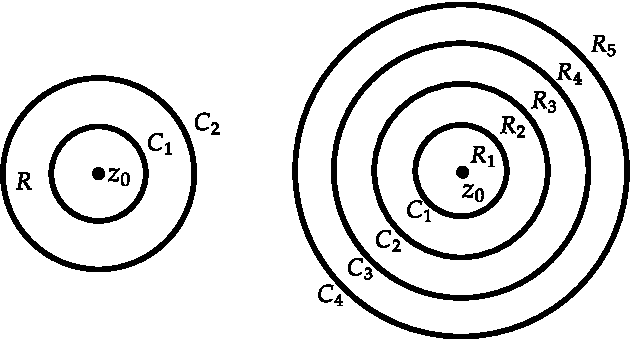
\includegraphics[height=3.7cm,width=7cm]{CN.01}
\end{figure}
The formulas for the coefficients are 
$$
a_{n}=\frac{1}{2 \pi i} \oint_{C} \frac{f(z) d z}{\left(z-z_{0}\right)^{n+1}}, \quad b_{n}=\frac{1}{2 \pi i} \oint_{C} \frac{f(z) d z}{\left(z-z_{0}\right)^{-n+1}},
$$
where $C$ is any simple closed curve surrounding $z_{0}$ and lying in $R$. However, this is not usually the easiest way to find a Laurent series. Like power series about a point, the Laurent series (about $z_{0}$ ) for a function in a given annular ring (about $z_{0}$ ) where the function is analytic, is unique, and we can find it by any method we choose. (See examples below.) If $f(z)$ has several isolated singularities, there are several annular rings, $R_{1}, R_{2}, \cdots$, in which $f(z)$ is analytic; then there are several different Laurent series for $f(z)$, one for each ring. The Laurent series which we usually want is the one that converges near $z_{0}$. If you have any doubt about the ring of convergence of a Laurent series, you can find out by testing the " $a$ " series and the "b" series separately.\\
\textbf{Singularity of Complex Function}\\
\textbf{Singular Point of an Analytic Function}\\\\
A point at which the function ceases to be analytic.\\
Example: $f(z)=\frac{1}{(z-2)}$ has a singularity at $\mathrm{z}=2$.\\
Different kinds of singularities exist. These are:\\
\textbf{Isolated Singularity}\\
A point $\mathrm{z}=\mathrm{z}_{0}$ is said to be isolated singularity of $f(z)$ if\\
(a) $f(z)$ is not analytic at $\mathrm{z}=\mathrm{z}_{0}$\\
(b) $f(z)$ is analytic in the neighbourhood of $\mathrm{z}=\mathrm{z}_{0}$ i.e. there exists a neighbourhood of $\mathrm{z}=\mathrm{z}_{0}$, containing no other singularity.
\begin{exercise}
	(i) Function $f(z)=\frac{1}{z}$ is analytic everywhere except at $\mathrm{z}=0$, therefore $\mathrm{z}=0$ is an isolated singularity.\\
	(ii) The function $f(z)=\frac{z+2}{(z-1)(z-2)(z-3)}$ has three isolated singularities at $z=1,2$ and 3 .
\end{exercise}
\textbf{Non-isolated Singularity}\\
\begin{align*}
f(z)&=\frac{1}{\left[\sin \frac{\pi}{z}\right]} \text { is not analytic when } \sin \frac{\pi}{z}=0 \Rightarrow \frac{\pi}{\mathrm{z}}=\mathrm{n} \pi \Rightarrow z=\frac{1}{n}(n=0,1,2,3 \ldots \ldots \ldots \ldots)\\
\text { Thus, } z&=0 \text { is an non-isolated singularity of } f(z) \text {, surrounded by a infinite number of other singularity } z=\frac{1}{n}\\
f(z)&=\frac{1}{\sin \pi / z} \text { has non-isolated singularity at } \mathrm{z}=0
\end{align*}
\textbf{Types of Isolated Singularity}\\
\begin{align*}
\text { If } \mathrm{f}(\mathrm{z}) \text { is an isolated singular point at } \mathrm{z}=\mathrm{a} &\text {, the we can expand } f(\mathrm{z}) \text { about } \mathrm{z}=\mathrm{a} \text { into laurent series as: }\\
\mathrm{f}(\mathrm{z})=\sum_{n=0}^{\infty} a_{n}(z-a)^{n}+\sum_{n=1}^{\infty} \frac{b_{n}}{(z-a)^{n}}&=\left[a_{0}+a_{1}(z-a)+a_{2}(z-a)^{2}+\ldots . .\right]+\left[\frac{b_{1}}{(z-a)}+\frac{b_{2}}{(z-a)^{2}}+\ldots . .\right]
\text{Therefore, three types of singularity are as follows.}
\end{align*}
\textbf{(1) Removable Singularity :} If the principal part of the Laurrent series expansion of $f(z)$ about $z=a$ contains no term i.e. if $b_{n}=0$ for all ' $n$ ', then $\mathrm{f}(\mathrm{z})$ has a removable singularity at $\mathrm{z}=\mathrm{a}$. In this case, Laurent series expansion is $f(z)=\sum_{n=0}^{\infty} a_{n}(z-a)^{n}$
\begin{exercise}
	Suppose $f(z)=\frac{\sin z}{z}$, then $\lim _{z \rightarrow 0}\left(\frac{\sin z}{z}\right)=1$, therefore, $z=0$ is a removable singularity of $f(z)$.\\
	Again, $\frac{\sin z}{z}=\frac{1}{z}\left(z-\frac{z^{3}}{3 !}+\ldots \ldots \ldots\right)=1-\frac{z^{2}}{3 !}+\frac{z^{4}}{5 !} \ldots \ldots$\\
	Since, there is no negative term in the laurent series expansion of $f(z)$ about $z=0$, hence $z=0$ is a removable singularity of $f(z)$.
\end{exercise}
\textbf{(2) Non-essential singularity or Pole:} If the principal part of the Laurrent series expansion of $f(z)$ about $z=$ a contains a finite number of terms, saym, i.e. $b_{n}=0$ for all $n>m$, then $f(z)$ has a non-essential singularity or a pole of order ' $m$ ' at $z=a$. A polc of order one is also known as simple pole.\\
Thus if $\mathrm{z}=\mathrm{a}$ is pole of order mof function $\mathrm{f}(\mathrm{z})$, then $\mathrm{f}(\mathrm{z})$ will have the Laurent series expansion of the form
$$
f(z)=\sum_{n=0}^{\infty} a_{n}\left(z-z_{0}\right)^{n}+\sum_{n=1}^{m} b_{n}\left(z-z_{0}\right)^{-n}
$$
Example : $f(z)=\frac{z}{(z-1)(z+2)^{2}}$ has a simple pole at $z=1$ and a pole of order 2 at $z=-2$.\\
\textbf{(3) Essential singularity: }If the principal part of the Laurrent series expansion of $f(z)$ about $z=a$, contains infinite number of terms i.e. $b_{n} \neq 0$ for infinitely many values of $n$, then $f(z)$ has an essential singularity at $z=a$.\\
Example : $f(z)=e^{1 / 2}$ has an essential singularity at $z=0$, since the expansion $e^{\frac{1}{z}}=1+\frac{1}{z}+\frac{1}{z^{2}} 2 !+\ldots . .$ is an infinite series of-ve powers of $\mathrm{z}$.\\
\begin{exercise}
	Examine the nature of singularity of the functions: (a) $\sin \left(\frac{1}{1-z}\right)$, (b) $(z-3) \sin \left(\frac{1}{z+2}\right)$.
\end{exercise}
\begin{answer}
	\begin{align*}
	\text{(a) }&\sin \left(\frac{1}{1-z}\right)=\frac{1}{1-z}-\frac{1}{(1-z)^{3} \cdot 3 !}+\frac{1}{(1-z)^{5} \cdot 5 !}-.
\text{	so, $z=1$ is an isolated essential singular point.}\\
\text { (b) }&(z-3) \sin \left(\frac{1}{z+2}\right)=(z-3)\left[\frac{1}{z+2}-\frac{1}{(z+2)^{3} \cdot 3 !}+\frac{1}{(z+2)^{5} .5 !}-\ldots \ldots . .\right] \text { so, } \mathrm{z}=-2 \text { is an isolated }\\
\text{essential point}
	\end{align*}
\end{answer}
\textbf{Zero of an Analytic Function}\\
\begin{align*}
\text{A zero of an analytic}&\text{ function $f(z)$ is a value of $z$ such that $f(z)=0$}\\
\text{An analytic function $\mathrm{f}(\mathrm{z})$}&\text{ is said to have a zero of order ' $\mathrm{m}$ ' at $\mathrm{z}=\mathrm{z}_{0}$ if $\mathrm{f}(\mathrm{z})$ is expressible as}\\
f(z)&\left(z-z_{0}\right)^{m} \phi(z)\\
\text{where $\phi(z)$ is analytic and $\phi\left(z_{0}\right) \neq 0$. }&\text{For $m=1, f(z)$ is said to have a simple zero at $z=z_{0}$}
\end{align*}
\textbf{Residue of Complex Fuction}\\
\textbf{Definition of residue at a pole:}\\
Let, $\mathrm{z}=$ a be a pole of order ' $m$ ' of $\mathrm{f}(\mathrm{z})$ and $\mathrm{C}_{1}$ is a circle of radius ' $r$ ' with center at $\mathrm{z}=$ a which does not contain singularities except $\mathrm{z}=\mathrm{a}$, then $\mathrm{f}(\mathrm{z})$ is analytic within the annular region $\mathrm{r}<|\mathrm{z}-\mathrm{a}|<\mathrm{R}$ can be expanded into Laurrent series within the annulur region as:
$$f(z)=\sum_{n=0}^{\infty} a_{n}(z-a)^{n}+\sum_{n=1}^{\infty} b_{n}(z-a)^{-n}$$
Co-efficient $\mathrm{b}_{1}$ is known as residue of $\mathrm{f}(\mathrm{z})$ at $\mathrm{z}=\mathrm{a}$ i.e. Res. $\mathrm{f}(\mathrm{z}=\mathrm{a})=\mathrm{b}_{1}=\frac{1}{2 \pi i} \oint f(z) d z$
\textbf{Methods of Finding Residues}\\
Method 1: Res. $f(z=a)=\underset{z \rightarrow a}{L t}(z-a) f(z)$\\
Method 2: If $f(z)=\frac{\phi(z)}{\psi(z)}$ where $\psi(a)=0$ but $\phi(a) \neq 0$, then $\operatorname{Res} . f(z=a)=\frac{\phi(a)}{\psi^{\prime}(a)}$\\
(b) Residue at a pole of order ' $n$ ':\\
Method 1: Res. $f(z=a)=\frac{1}{(n-1) !}\left\{\frac{d^{n-1}}{d z^{n-1}}\left[(z-a)^{n} f(z)\right]\right\}_{z=a}$\\
Method 2: First put $z+a=t$ and expand it into series, then Res. $f(z=a)=$ co-efficient of $1 / t$.\\
(c ) Residue at $\mathrm{z}=\infty$ : Res. $f(z=\infty) \underset{z \rightarrow \infty}{L t}[-z f(z)]$
\begin{exercise}
	 Find the singular points of the following function and the corresponding residues:\\
	(a) $f(z)=\frac{1-2 z}{z(z-1)(z-2)}$\quad
	(b) $f(z)=\frac{z^{2}}{z^{2}+a^{2}}$\quad
	(c) $f(z)=z^{2} e^{1 / z}$
\end{exercise}
\begin{answer}
	\begin{align*}
	\text{(a )}f(z)&=\frac{1-2 z}{z(z-1)(z-2)} \Rightarrow \text { Poles }: z=0, z=1, z=2\\
	\text{Res. }f(z=0)&=\operatorname{Lt}_{z \rightarrow 0}(z-0) f(z)=\operatorname{Lt}_{z \rightarrow 0} \frac{1-2 z}{(z-1)(z-2)}=\frac{1}{2}.\\
	\text{Res. } f(z=1)&=L_{z \rightarrow 1}(z-1) f(z)=L_{z \rightarrow 1} \frac{1-2 z}{z(z-2)}=1\\
	\text{Res. }f(z=2)&=\underset{z \rightarrow 2}{L t}(z-2) f(z)=\underset{z \rightarrow 2}{L t} \frac{1-2 z}{z(z-1)}=-\frac{3}{2}\\\\
\text{	(b) }f(z)&=\frac{z^{2}}{z^{2}+a^{2}} \Rightarrow\text{ Poles : }z=i a, z=-i a\\
	\text { Res. } f(z=i a)&=\left(\frac{z^{2}}{2 z}\right)_{z=i a}=\frac{1}{2} i a ; \operatorname{Res} . f(z=-i a)=\left(\frac{z^{2}}{2 z}\right)_{z=-i a}=-\frac{1}{2} i a\\\\
	\text{(c) }f(z)&=z^{2} e^{1 / z}=z^{2}\left[1+\frac{1}{z}+\frac{1}{z^{2} \cdot 2 !}+\frac{1}{z^{3} \cdot 3 !}+\ldots \ldots .\right] \Rightarrow\text{ Poles :} z=0\\
	\text{Res. }f(z=0)&=\text{ Coefficient of }\frac{1}{z}=\frac{1}{3 !}=\frac{1}{6}
	\end{align*}
\end{answer}
\textbf{Cauchy's Residue Theorem :}
If $\mathrm{f}(\mathrm{z})$ in single-valued and analytic in a closed curve ' $\mathrm{C}$ ', except at a finite number of poles within ' $\mathrm{C}$, then $\oint_{C} \mathrm{f}(\mathrm{z}) \mathrm{dz}=2 \pi \mathrm{i}$ (sum of the residues at poles within ' $\mathrm{C}^{\prime}$ )
\begin{exercise}
	Evaluate the integral: $\oint_{C} \frac{4-3 z}{z(z-1)(z-3)} d z$ where $|z|=\frac{3}{2}$
\end{exercise}
\begin{answer}
	\begin{align*}
	\hat{f}(z)&=\frac{4-3 z}{z(z-1)(z-3)} \Rightarrow\text{ Poles : }z=0, z=1, z=3\\
\intertext{	But, the given contour is circle centered at the origin and radius $3 / 2$ units.} 
\text{Therefore, only $z=0$ }&\text{and $z=1$ within the contour.}\\
	I&=2 \pi i[\operatorname{Re} s . f(z=0)+\operatorname{Re} s . f(z=1)]=2 \pi i\left[\frac{4}{3}-\frac{1}{2}\right]=\frac{5 \pi i}{3}
	\end{align*}
\end{answer}
\begin{exercise}
	Evaluate the integral: $\oint_{C} \frac{e^{2 z}+z^{2}}{(z-1)^{5}} d z$ where $|z|=2$
\end{exercise}
\begin{answer}
	\begin{align*}
	\begin{aligned}
	f(z)&=\frac{e^{2 z}+z^{2}}{(z-1)^{5}} \Rightarrow \text { Poles }: z=1(\text { order } 5) \\
	I&=2 \pi i \times \operatorname{Re} s . f(z=1)=2 \pi i \times \frac{1}{4 !} \frac{d^{4}}{d z^{4}}\left[e^{2 z}+z^{2}\right]_{z=1}=2 \pi i \times \frac{2 e^{2}}{3}=\frac{4 \pi i e^{2}}{3} .
	\end{aligned}
	\end{align*}
\end{answer}
\textbf{Definite Integrals of Trigonometric Functions of $\cos\theta$ and $\sin\theta$ : (Integration round the unit circle)} :\\
	Method: Consider the contour to be a circle centered at the origin and having radius one unit i.e. $|\mathrm{z}|=1$
\begin{align*}
	\text{Assume, }z&=e^{i \theta} \Rightarrow d z=i e^{i \theta} d \theta \Rightarrow d \theta=\frac{d z}{i z}\\
	\text{Therefore, }\cos \theta&=\frac{e^{i \theta}+e^{-i \theta}}{2}=\frac{1}{2}\left(z+\frac{1}{z}\right)
	 \text{and }\sin \theta=\frac{e^{i \theta}-e^{-i \theta}}{2 i}=\frac{1}{2 i}\left(z-\frac{1}{z}\right)\\
	 \text { and the limit will be changed from }& 0 \rightarrow 2 \pi \text { to } \oint_{C}
\end{align*}
The replacements regarding $\cos \theta$ and $\sin \theta$ is to be done only in the denominator of the given integral.
\begin{exercise}
	Evaluate the integral: $\int_{0}^{2 \pi} \frac{d \theta}{a+b \cos \theta} ; \quad a>b>0$
\end{exercise}
\begin{answer}
	\begin{align*}
	\int_{0}^{2 \pi} \frac{d \theta}{a+b \cos \theta}&=\int_{0}^{2 \pi} \frac{d z / i z}{a+b\left(\frac{z^{2}+1}{2 z}\right)}=\int_{0}^{2 \pi} \frac{2 d z}{i\left(b z^{2}+2 a z+b\right)}\\
	\text { The singular points are at } \Rightarrow z&=\alpha=\frac{-a+\sqrt{a^{2}-b^{2}}}{b} \quad \& \quad z=\beta=\frac{-a-\sqrt{a^{2}-b^{2}}}{b}\\
	\intertext{The singular point $z=\beta$ will lie outside the unit circle as $a>b>0$ while the singular point $z=\alpha$ will lie inside the unit circle which is a simple pole.}\\
	\text { Res. } f(z=\alpha)=\lim _{z \rightarrow \alpha}(z-\alpha) f(z)&=\lim _{z \rightarrow \alpha} \frac{2}{i b} \frac{(z-\alpha)}{(z-\alpha)(z-\beta)}=\frac{2}{i b(\alpha-\beta)}=\frac{2}{i b} \times \frac{b}{2 \sqrt{a^{2}-b^{2}}}=\frac{1}{i \sqrt{a^{2}-b^{2}}}\\
\text { Therefore,  }\text{by cauchy Residue theorem.}&\\
I=2 \pi i \times \text { Residue }&=2 \pi \mathrm{i} \times \frac{1}{i \sqrt{a^{2}-b^{2}}}=\frac{2 \pi}{\sqrt{a^{2}-b^{2}}}
	\end{align*}
\end{answer}


\textbf{ Evaluation of improper integrals between the limit $-\infty$ to $+\infty$ : }\\
\textbf{Theorem I:}\\
\begin{align*}
\text{If $f(x)$ contain}&\text{ only polynomial terms}\\
\text{then }f(x)&=f(x) \\
\rightarrow&\text{ find singular points}\\
\rightarrow&\text{ check point lie in upper half}
\intertext{\textbf{A.}\quad If singular point lie on imaginary axis}
\int\limits_{-\infty}^{\infty}f(z)dz&=\int\limits_{-\infty}^{\infty}f(x)dx
=2\pi i[\Sigma \text{ Res}]-\left( \stackrel{\text{lim}}{z\rightarrow \infty}\quad zf(x)\right) x\pi i
\intertext{\textbf{B.}\quad If singular point lie on real axis }
\int\limits_{-\infty}^{\infty}f(x)dx=&
\int\limits_{-\infty}^{\infty}f(z)dz=\pi i[\Sigma \text{ Res}]-\pi i \left[\stackrel{\text{lim}}{z\rightarrow \infty}\quad zf(z) \right] 
\end{align*}
\textbf{Theorem II:}
\begin{align*}
\intertext{If $f(x)$ contains sine and cosine function along with polynomial function rule is same, except second term which is $0$ in this case.}
\intertext{\textbf{A.}\quad If singular point lie on imaginary axis}\\
\int\limits_{-\infty}^{\infty}f(z)dz&=\int\limits_{-\infty}^{\infty}f(x)dx
=2\pi i[\Sigma \text{ Res}]
\intertext{\textbf{B.}\quad If singular point lie on real axis }
\int\limits_{-\infty}^{\infty}f(x)dx&=
\int\limits_{-\infty}^{\infty}f(z)dz=\pi i[\Sigma \text{ Res}]
\end{align*}
\newpage
\begin{abox}
	Practise Set-1
	\end{abox}
\begin{enumerate}[label=\color{ocre}\textbf{\arabic*.}]
	\item The value of the integral $\int_{C} d z z^{2} e^{z}$, where $C$ is an open contour in the complex $z$-plane as shown in the figure below, is:
	{\exyear{NET/JRF(JUNE-2011)}}
	\begin{figure}[H]
		\centering
		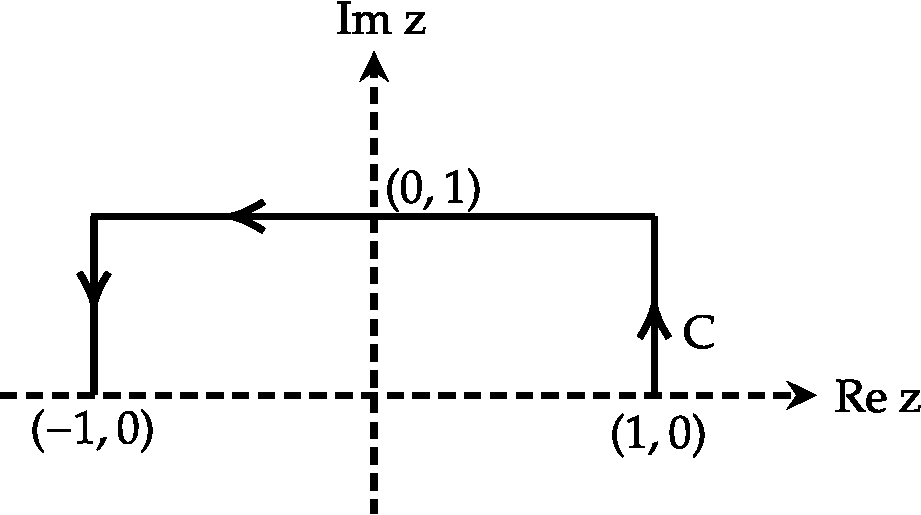
\includegraphics[height=5cm,width=9cm]{diagram-20211005-crop}
	\end{figure}
	\begin{tasks}(4)
		\task[\textbf{A.}] $\frac{5}{e}+e$
		\task[\textbf{B.}] $e-\frac{5}{e}$
		\task[\textbf{C.}] $\frac{5}{e}-e$
		\task[\textbf{D.}] $-\frac{5}{e}-e$
	\end{tasks}
	\begin{answer}
		\begin{align*}
		\intertext { If we complete the contour, then by Cauchy integral theorem }
		\int_{-1}^{1} d z z^{2} e^{z}+\int_{C} d z z^{2} e^{z}&=0 \Rightarrow \int_{C} d z z^{2} e^{z}=-\int_{-1}^{1} d z z^{2} e^{z}\\&=-\left[z^{2} e^{z}-2 z e^{2}+2 e^{2}\right]_{-1}^{1}=\frac{5}{e}-e
		\end{align*}
		So the correct answer is \textbf{Option (C)}
	\end{answer}
	\item Which of the following is an analytic function of the complex variable $z=x+i y$ in the domain $|z|<2 ?$
	{\exyear{NET/JRF(JUNE-2011)}}
	\begin{tasks}(2)
		\task[\textbf{A.}] $(3+x-i y)^{7}$
		\task[\textbf{B.}] $(1+x+i y)^{4}(7-x-i y)^{3}$
		\task[\textbf{C.}] $(1-x-i y)^{4}(7-x+i y)^{3}$
		\task[\textbf{D.}] $(x+i y-1)^{1 / 2}$
	\end{tasks}
	\begin{answer}
		Put $z=x+i y .$ If $\bar{z}=x-i y$ appears in any of the expressions then that expression is non-analytic. For option (D) we have a branch point singularity as the power is $\frac{1}{2}$ which is fractional. Hence only option (B) is analytic.\\\\
		So the correct answer is \textbf{Option (B)}
	\end{answer}
	\item The first few terms in the Laurent series for $\frac{1}{(z-1)(z-2)}$ in the region $1 \leq|z| \leq 2$ and around $z=1$ is
	{\exyear{NET/JRF(JUNE-2012)}}
	\begin{tasks}(1)
		\task[\textbf{A.}] $\frac{1}{2}\left[1+z+z^{2}+\ldots\right]\left[1+\frac{z}{2}+\frac{z^{2}}{4}+\frac{z^{3}}{8}+\ldots .\right]$
		\task[\textbf{B.}] $\frac{1}{1-z}-z-(1-z)^{2}+(1-z)^{3}+\ldots .$
		\task[\textbf{C.}] $\frac{1}{\mathrm{z}^{2}}\left[1+\frac{1}{\mathrm{z}}+\frac{1}{\mathrm{z}^{2}}+\ldots .\right]\left[1+\frac{2}{\mathrm{z}}+\frac{4}{\mathrm{z}^{2}}+\ldots . .\right]$
		\task[\textbf{D.}]  $2(z-1)+5(z-1)^{2}+7(z-1)^{3}+\ldots$
	\end{tasks}
	\begin{answer}
		\begin{align*}
		\frac{1}{(z-1)(z-2)}&=\frac{1}{z-2}-\frac{1}{z-1}=\frac{1}{1-z}+\frac{1}{(z-1)-1}\\&=\frac{1}{1-z}-(1+(1-z))^{-1}\\
		&=\frac{1}{1-z}-\left[1+(1-z)+\frac{(-1)(-2)}{2 !}(1-z)^{2}+\frac{(-1)(-2)(-3)}{3 !}(1-z)^{3} \ldots\right]\\
		&=\frac{1}{1-z}-\left[z+(1-z)^{2}-(1-z)^{3}+\ldots . .\right]
		\end{align*}
		So the correct answer is \textbf{Option (B)}
	\end{answer}
	\item Let $u(x, y)=x+\frac{1}{2}\left(x^{2}-y^{2}\right)$ be the real part of analytic function $f(z)$ of the complex variable $z=x+i y$. The imaginary part of $f(z)$ is
	{\exyear{NET/JRF(JUNE-2012)}}
	\begin{tasks}(4)
		\task[\textbf{A.}] $y+x y$
		\task[\textbf{B.}] $x y$
		\task[\textbf{C.}] $y$
		\task[\textbf{D.}] $y^{2}-x^{2}$
	\end{tasks}
	\begin{answer}
		\begin{align*}
		u(x, y)&=x+\frac{1}{2}\left(x^{2}-y^{2}\right), v(x, y)=?\\
		\text{Check }\frac{\partial u}{\partial x}&=\frac{\partial v}{\partial y}\text{ and } \frac{\partial u}{\partial y}=-\frac{\partial v}{\partial x}\\
		\Rightarrow \frac{\partial u}{\partial x}&=\frac{\partial v}{\partial y}, \quad \frac{\partial v}{\partial y}=1+x, \\ v&=y+x y+f(x)\\
		\frac{\partial u}{\partial y}&=-\frac{\partial v}{\partial x} \Rightarrow \frac{\partial v}{\partial x}=+y, \\ v&=y x+f(y)\\
		y+x y+f(x)&=y x+f(y)\\
		\text{If }f(x)&=0\quad \quad
		f(y)=y\\
		v&=x y+y
		\end{align*}
		So the correct answer is \textbf{Option (A)}
	\end{answer}
	\item The value of the integral $\int_{C} \frac{z^{3} d z}{\left(z^{2}-5 z+6\right)}$, where $C$ is a closed contour defined by the equation $2|z|-5=0$, traversed in the anti-clockwise direction, is
	{\exyear{NET/JRF(DEC-2012)}}
	\begin{tasks}(4)
		\task[\textbf{A.}] $-16 \pi i$
		\task[\textbf{B.}] $16 \pi \mathrm{i}$
		\task[\textbf{C.}] $8 \pi i$
		\task[\textbf{D.}] $2 \pi i$
	\end{tasks}
	\begin{answer}
		\begin{align*}
		z^{2}-5 z+6&=0 \Rightarrow z^{2}-2 z-3 z+6\\&=0 \Rightarrow z(z-2)-3(z-2)=0 \Rightarrow z=3,2\\
		2|z|&=5 \Rightarrow|z|=2.5,\text{ only 2 will be inside.}\\
		\text{Residue }&=\left.(z-2) \frac{z^{3}}{(z-3)(z-2)}\right|_{z=2}=\frac{8}{2-3}\\&=-8 \Rightarrow \int \frac{z^{3} d z}{z^{2}-5 z+6}=2 \pi i(-8)=-16 \pi i
		\end{align*}
		So the correct answer is \textbf{Option (A)}
	\end{answer}
	\item  With $z=x+i y$, which of the following functions $f(x, y)$ is NOT a (complex) analytic function of $z$ ?
	{\exyear{NET/JRF(JUNE-2013)}}
	\begin{tasks}(1)
		\task[\textbf{A.}] $f(x, y)=(x+i y-8)^{3}\left(4+x^{2}-y^{2}+2 i x y\right)^{7}$
		\task[\textbf{B.}] $f(x, y)=(x+i y)^{7}(1-x-i y)^{3}$
		\task[\textbf{C.}] $f(x, y)=\left(x^{2}-y^{2}+2 i x y-3\right)^{5}$
		\task[\textbf{D.}] $f(x, y)=(1-x+i y)^{4}(2+x+i y)^{6}$
	\end{tasks}
	\begin{answer}
		\begin{align*}
		f(x, y)&=(1-x+i y)^{4}(2+x+i y)^{6}\\&=\{1-(x-i y)\}^{4}(2+x+i y)^{6}\\
		\text{Due to present of }\bar{z}&=(x-i y)
		\end{align*}
		So the correct answer is \textbf{Option (D)}
	\end{answer}
	\item  Which of the following functions cannot be the real part of a complex analytic function of $z=x+i y ?$
	{\exyear{NET/JRF(DEC-2013)}}
	\begin{tasks}(4)
		\task[\textbf{A.}] $x^{2} y$
		\task[\textbf{B.}]  $x^{2}-y^{2}$
		\task[\textbf{C.}] $x^{3}-3 x y^{2}$
		\task[\textbf{D.}] $3 x^{2} y-y-y^{3}$
	\end{tasks}
	\begin{answer}
		\begin{align*}
		\intertext{ Let $x^{2} y$ be real part of a complex function. Use Milne Thomson's method to write analytic complex function. The real part of that function should be (1) but that is not the case. So this cannot be real part of an analytic function. Also,}
		z^{2}&=(x+i y)^{2}=x^{2}-y^{2}+2 i x y,\text{ Real part option (2)}\\
		z^{3}&=(x+i y)^{3}=x^{3}-i y^{3}+3 i x y(x+i y)\\
		&=x^{3}-i y^{3}+3 i x^{2} y-3 x y^{2},\text{ Real part option (3)}
		\end{align*}
		So the correct answer is \textbf{Option (A)}
	\end{answer}
	\item  Given that the integral $\int_{0}^{\infty} \frac{d x}{y^{2}+x^{2}}=\frac{\pi}{2 y}$, the value of $\int_{0}^{\infty} \frac{d x}{\left(y^{2}+x^{2}\right)^{2}}$ is
	{\exyear{NET/JRF(DEC-2013)}}
	\begin{tasks}(4)
		\task[\textbf{A.}] $\frac{\pi}{y^{3}}$
		\task[\textbf{B.}] $\frac{\pi}{4 y^{3}}$
		\task[\textbf{C.}]  $\frac{\pi}{8 y^{3}}$
		\task[\textbf{D.}] $\frac{\pi}{2 y^{3}}$
	\end{tasks}
	\begin{answer}
		\begin{align*}
		\int_{0}^{\infty} \frac{d x}{\left(y^{2}+x^{2}\right)^{2}}&=\frac{1}{2} \int_{-\infty}^{\infty} \frac{d x}{\left(y^{2}+x^{2}\right)^{2}},\text{ pole is of }2^{\text {nd }}\text{ order at }x=i y,\text{ residue }=1 /\left(4 i y^{3}\right)\\
		\text{Integral }&=\left(\frac{1}{2}\right)(2 \pi i) \frac{1}{4 i y^{3}}=\frac{\pi}{\left(4 y^{3}\right)}
		\end{align*}
	\end{answer}
	\item If $C$ is the contour defined by $|z|=\frac{1}{2}$, the value of the integral
	$$
	\oint_{C} \frac{d z}{\sin ^{2} z}
	$$
	is
	{\exyear{NET/JRF(JUNE-2014)}}
	\begin{tasks}(4)
		\task[\textbf{A.}] $\infty$
		\task[\textbf{B.}] $2 \pi i$
		\task[\textbf{C.}] 0
		\task[\textbf{D.}] $\pi i$
	\end{tasks}
	\begin{answer}
		\begin{align*}
		f(z)&=\frac{1}{\sin ^{2} z} \quad\left(|z|=\frac{1}{2}\right)\\
		\sin z&=z-\frac{z^{3}}{\lfloor 3}+\frac{z^{5}}{\lfloor 5} \ldots . \Rightarrow \frac{1}{\sin ^{2} z}=\frac{1}{\left(z-\frac{z^{3}}{\frac{3}{3}}+\frac{z^{5}}{5} \cdots\right)^{2}}\\
		\Rightarrow \frac{1}{\sin ^{2} z}&=\frac{1}{z^{2}}\left[1-\frac{z^{2}}{\lfloor 3}+\frac{z^{4}}{\lfloor 5} \ldots .\right]^{-2} \Rightarrow \oint_{C} \frac{d z}{\sin ^{2} z}=0
		\end{align*}
		So the correct answer is \textbf{Option (C)}
	\end{answer}
	\item The principal value of the integral $\int_{-\infty}^{\infty} \frac{\sin (2 x)}{x^{3}} d x$ is
	{\exyear{NET/JRF(DEC-2014)}}
	\begin{tasks}(4)
		\task[\textbf{A.}] $-2 \pi$
		\task[\textbf{B.}]  $-\pi$
		\task[\textbf{C.}] $\pi$
		\task[\textbf{D.}]  $2 \pi$
	\end{tasks}
	\begin{answer}
		\begin{align*}
		\text{Let }f(z)&=\frac{e^{i 2 z}}{z^{3}}\\
		\lim _{2 \rightarrow 0}(z-0)^{3} f(z)&=\lim _{z \rightarrow 0}(z-0)^{3} \frac{e^{i 2 z}}{z^{3}}\\&=1(\text{ finite and }\neq 0) \Rightarrow z=0 \text{is pole of order 3} .\\
		\text{Residue }R&=\frac{1}{2 !} \lim _{z \rightarrow 0} \frac{d^{2}}{d z^{2}}\left[(z-0)^{3} \frac{e^{i 2 z}}{z^{3}}\right]=-2\\
		\Rightarrow \int_{-\infty}^{\infty} f(x) d x&=\pi i \Sigma R=\pi i(-2)=-2 \pi i \Rightarrow \operatorname{Im} .\text{ Part }\\&=-2 \pi \Rightarrow \int_{-\infty}^{\infty} f(x) d x=-2 \pi
		\end{align*}
		So the correct answer is \textbf{Option (A)}
	\end{answer}
	\item The Laurent series expansion of the function $f(z)=e^{2}+e^{1 / 2}$ about $z=0$ is given by
	{\exyear{NET/JRF(DEC-2014)}}
	\begin{tasks}(2)
		\task[\textbf{A.}] $\sum_{n=-\infty}^{\infty} \frac{z^{n}}{n !}$ for all $|z|<\infty$
		\task[\textbf{B.}] $\sum_{n=0}^{\infty}\left(z^{n}+\frac{1}{z^{n}}\right) \frac{1}{n !}$ only if $0<|z|<1$
		\task[\textbf{C.}] $\sum_{n=0}^{\infty}\left(z^{n}+\frac{1}{z^{n}}\right) \frac{1}{n !}$ for all $0<|z|<\infty$
		\task[\textbf{D.}]  $\sum_{n=-\infty}^{\infty} \frac{z^{n}}{n !}$ only if $|z|<1$
	\end{tasks}
	\begin{answer}
		\begin{align*}
		e^{z}&=\left(1+z+\frac{z^{2}}{2 !}+\ldots\right)=\sum_{n=0}^{\infty} \frac{z^{n}}{n !}\text{ and }e^{1 / z}\\&=1+\frac{1}{z}+\frac{1}{2 !} \frac{1}{z^{2}}+\ldots .=\sum_{n=0}^{\infty} \frac{1}{z^{n} n !}\\
		\Rightarrow f(z)&=\left(e^{z}+e^{1 / 2}\right)=\sum_{n=0}^{\infty}\left(z^{n}+\frac{1}{z^{n}}\right) \frac{1}{n !},\text{ for all }0<|z|<\infty
		\end{align*}
		So the correct answer is \textbf{Option (C)}
	\end{answer}
	\item Consider the function $f(z)=\frac{1}{z} \ln (1-z)$ of a complex variable $z=r e^{i \theta}(r \geq 0, \quad-\infty<\theta<\infty)$. The singularities of $f(z)$ are as follows:
	{\exyear{NET/JRF(DEC-2014)}}
	\begin{tasks}(1)
		\task[\textbf{A.}]  Branch points at $z=1$ and $z=\infty$; and a pole at $z=0$ only for $0 \leq \theta<2 \pi$
		\task[\textbf{B.}] Branch points at $z=1$ and $z=\infty$; and a pole at $z=0$ for all $\theta$ other than $0 \leq \theta<2 \pi$
		\task[\textbf{C.}] Branch points at $z=1$ and $z=\infty$; and a pole at $z=0$ for all $\theta$
		\task[\textbf{D.}] Branch points at $z=0, z=1$ and $z=\infty$.
	\end{tasks}
	\begin{answer}
		\begin{align*}
		\text{For }f(z)&=\frac{1}{z} \ln (1-z)=\frac{1}{z}\left(-z-\frac{z^{2}}{2}-\frac{z^{3}}{3}-\ldots . .\right)\\&=-1-\frac{z}{2}-\frac{z^{2}}{3}-\ldots .
		\intertext{There is no principal part and when $z \rightarrow 0, f(z)=-1 .$ So there is removable singularity at $z=0$. Also $z=1$ and $z=\infty$ is Branch point.}
		\end{align*}
		None of the above is correct
	\end{answer}
	\item  The value of integral $\int_{-\infty}^{\infty} \frac{d x}{1+x^{4}}$
	{\exyear{NET/JRF(JUNE-2015)}}
	\begin{tasks}(4)
		\task[\textbf{A.}] $\frac{\pi}{\sqrt{2}}$
		\task[\textbf{B.}] $\frac{\pi}{2}$
		\task[\textbf{C.}] $\sqrt{2} \pi$
		\task[\textbf{D.}] $2 \pi$
	\end{tasks}
	\begin{answer}
		\begin{align*}
		\int_{-\infty}^{\infty} \frac{d z}{1+z^{4}} \quad \because|z|=R\\
		\text{Now, pole }z&=e^{(2 n+1) \frac{\pi}{4}}\\
		n&=0, \quad \Rightarrow z_{0}=e^{\frac{i \pi}{4}}=\frac{1}{\sqrt{2}}+i \frac{1}{\sqrt{2}}, n\\&=2 \Rightarrow z_{2}=\frac{-1}{\sqrt{2}}-i \frac{1}{\sqrt{2}}\\
		n&=1 \Rightarrow z_{1}=e^{\frac{i 3 \pi}{4}}=\frac{-1}{\sqrt{2}}+i \frac{1}{\sqrt{2}}, n\\&=3 \Rightarrow z_{3}=+\frac{1}{\sqrt{2}}-i \frac{1}{\sqrt{2}}
		\intertext{only $z_{0}$ and $z_{1}$ lies in contour}
		\text{i.e., residue at }\left(z=e^{\frac{i \pi}{4}}\right)&=\frac{1}{4}\left(-\frac{1}{\sqrt{2}}-i \frac{1}{\sqrt{2}}\right)\\
		\text{residue at }\left(z=e^{\frac{i 3 \pi}{4}}\right)&=\frac{1}{4}\left(\frac{1}{\sqrt{2}}-i \frac{1}{\sqrt{2}}\right)\\
		\text{now }\int_{-\infty}^{\infty} \frac{d x}{x^{4}+1}&=2 \pi i \Sigma \operatorname{Re} S=\frac{\pi}{\sqrt{2}}
		\end{align*}
		So the correct answer is \textbf{Option (A)}
	\end{answer}
	\item  The function $\frac{Z}{\sin \pi z^{2}}$ of a complex variable $z$ has
	{\exyear{NET/JRF(DEC-2015)}}
	\begin{tasks}(1)
		\task[\textbf{A.}] A simple pole at 0 and poles of order 2 at $\pm \sqrt{n}$ for $n=1,2,3 \ldots$
		\task[\textbf{B.}] A simple pole at 0 and poles of order 2 at $\pm \sqrt{n}$ and $\pm i \sqrt{n}$ for $n=1,2,3 \ldots$
		\task[\textbf{C.}] Poles of order 2 at $\pm \sqrt{n}, n=0,1,2,3 \ldots$
		\task[\textbf{D.}] Poles of order 2 at $\pm n, n=0,1,2,3 \ldots$
	\end{tasks}
	\begin{answer}
		\begin{align*}
		f(z)&=\frac{z}{\sin \pi z^{2}}=\frac{z}{\pi z^{2} \frac{\sin \pi z^{2}}{\pi z^{2}}}\\
		\text{	at }z&=0,\text{ it is a simple pole since,} \lim _{z \rightarrow 0} \frac{\sin \pi z^{2}}{\pi z^{2}}=1\\
		\text{Also, }\sin \pi z^{2}&=\sin n \pi \Rightarrow \pi \mathrm{z}^{2}\\&=\pm n \pi, z=\pm \sqrt{n}, \pm i \sqrt{n}\\
		\lim _{z \rightarrow \sqrt{n}}&(z-\sqrt{n})^{2} \cdot \frac{z}{\sin \pi z^{2}}, \text{exists. So its pole of order 2}
		\end{align*}
		So the correct answer is \textbf{Option (B)}
	\end{answer}
	\item The value of the contour integral $\frac{1}{2 \pi i} \oint_{C} \frac{e^{4 z}-1}{\cosh (z)-2 \sinh (z)} d z$ around the unit circle $C$ traversed in the anti-clockwise direction, is
	{\exyear{NET/JRF(JUNE-2016)}}
	\begin{tasks}(4)
		\task[\textbf{A.}] 0
		\task[\textbf{B.}] 2
		\task[\textbf{C.}] $\frac{-8}{\sqrt{3}}$
		\task[\textbf{D.}] $-\tanh \left(\frac{1}{2}\right)$
	\end{tasks}
	\begin{answer}
		\begin{align*}
		f(z)&=\frac{e^{4 z}-1}{\cosh z-2 \sinh z}=\frac{e^{4 z}-1}{\frac{e^{2}+e^{-z}}{2}-\left(e^{z}-e^{-z}\right)}\\&=\frac{e^{42}-1}{-\frac{e^{z}}{2}+\frac{3}{2} e^{-z}}\\
		\Rightarrow f(z)&=\frac{2 e^{2}\left(e^{4 z}-1\right)}{\left(3-e^{2 z}\right)}=\frac{2\left(e^{5 z}-e^{z}\right)}{\left(3-e^{2 z}\right)}\\
		\text{For pole at }z&=z_{0}, 3-e^{2 \xi_{0}}=0 \Rightarrow e^{2 z_{0}}\\&=3 \Rightarrow z_{0}=\frac{\ln 3}{2}
		\intertext{It has simple pole at $z_{0}$}
		\operatorname{Re}\left(z_{0}\right)&=\lim _{z \rightarrow z_{0}}\left(z-z_{0}\right) f(z)=\lim _{2 \rightarrow z_{0}}\left(z-z_{0}\right) \frac{2\left(e^{5 z}-e^{2}\right)}{3-e^{22}}\\
		&=\lim _{z \rightarrow z_{0}} \frac{\left(z-z_{0}\right) \times 2\left(5 e^{5 z}-e^{z}\right)+2\left(e^{5 z}-e^{z}\right) \times 1}{-2 e^{2 z}}\\&=-\left(\frac{e^{5 z_{0}}-e^{z_{0}}}{e^{2 z_{0}}}\right)\\
		&=-\left(\frac{(\sqrt{3})^{5}-\sqrt{3}}{3}\right)=-\left(\frac{9 \sqrt{3}-\sqrt{3}}{3}\right)=-\frac{8}{\sqrt{3}}\\
		\frac{1}{2 \pi i} \oint f(z) d z&=\frac{1}{2 \pi i} \times 2 \pi i \sum\text{ Residue } =-\frac{8}{\sqrt{3}}
		\end{align*}
		So the correct answer is \textbf{Option (C)}
	\end{answer}
	\item  Let $u(x, y)=e^{a x} \cos (b y)$ be the real part of a function $f(z)=u(x, y)+i v(x, y)$ of the complex variable $z=x+i y$, where $a, b$ are real constants and $a \neq 0 .$ The function $f(z)$ is complex analytic everywhere in the complex plane if and only if
	{\exyear{NET/JRF(JUNE-2017)}}
	\begin{tasks}(4)
		\task[\textbf{A.}] $b=0$
		\task[\textbf{B.}] $b=\pm a$
		\task[\textbf{C.}] $b=\pm 2 \pi a$
		\task[\textbf{D.}]  $b=a \pm 2 \pi$
	\end{tasks}
	\begin{answer}
		\begin{align*}
		\intertext{The function $f(z)$ will be analytic everywhere in the complex plane if and only if it satisfies the Cauchy Riemann equation in that region.}
		\Rightarrow \frac{\partial u}{\partial x}&=\frac{\partial v}{\partial y}\text{ and } \frac{\partial u}{\partial y}=-\frac{\partial v}{\partial x}\\
		\text{Hence }a e^{a x} \cos (b y)&=\frac{\partial v}{\partial y}\hspace{2cm}\text{(i)}\\
		\text{and }b e^{a x} \sin (b y)&=\frac{\partial v}{\partial x}\hspace{2cm}\text{(ii)}
		\intertext{From equation (i)}
		v(x, y)&=\frac{a e^{a x} \sin (b y)}{b}+c(y)\hspace{2cm}\text{(iii)}
		\intertext{Differentiating partially with $x$ gives}
		\frac{\partial v}{\partial x}&=\frac{a^{2} e^{a x} \sin (b y)}{b}\hspace{2cm}\text{(iv)}
		\intertext{From equation (iii) and (iv)}
		b e^{a x} \sin (b y)&=\frac{a^{2} e^{a x} \sin (b y)}{b}\\
		\Rightarrow b^{2}&=a^{2} \Rightarrow b=\pm a
		\end{align*}
		So the correct answer is \textbf{Option (B)}
	\end{answer}
	\item  The integral $\oint_{\Gamma} \frac{z e^{i \pi z / 2}}{z^{2}-1} d z$ along the closed contour $\Gamma$ shown in the figure is
	{\exyear{NET/JRF(JUNE-2017)}}
	\begin{figure}[H]
		\centering
		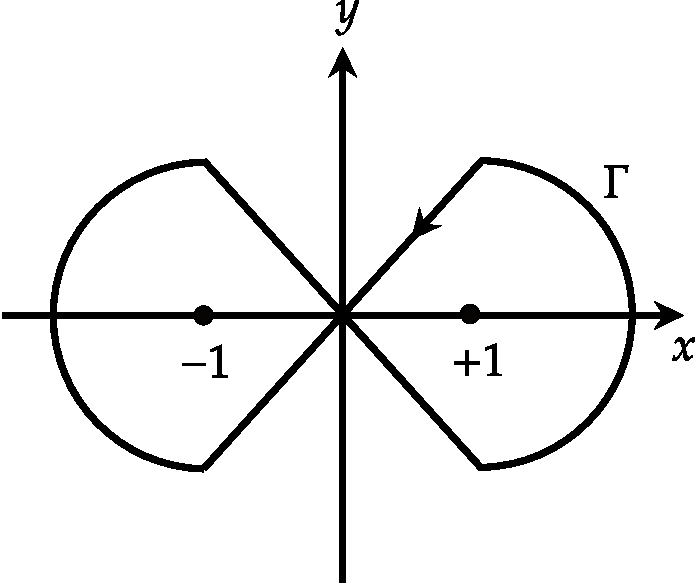
\includegraphics[height=4cm,width=5cm]{diagram-20211005(19)-crop}
	\end{figure}
	\begin{tasks}(4)
		\task[\textbf{A.}] 0
		\task[\textbf{B.}] $2 \pi$
		\task[\textbf{C.}] $-2 \pi$
		\task[\textbf{D.}] $4 \pi i$
	\end{tasks}
	\begin{answer}
		\begin{align*}
		f(z)&=\frac{z e^{i z \pi / 2}}{(z+1)(z-1)}\\
		\text{For }z&=+1\text{ anti-clockwise}\\
		I&=2 \pi i \lim _{z \rightarrow 1} \frac{z e^{i \pi z / 2}}{(z+1)}=\frac{2 \pi i}{2} e^{i \pi / 2}=\pi i e^{i \pi / 2}\\
		\text{For }z&=-1\\
		I&=-2 \pi i \lim _{z \rightarrow-1} \frac{z e^{i \pi z / 2}}{(z-1)}=-2 \pi i \times \frac{(-1) e^{-i \pi / 2}}{(-2)}=-\pi i e^{-i \pi / 2}\\
		\text{Integral }&=\pi i \frac{\left(e^{i \pi / 2}-e^{-i \pi / 2}\right)}{2 i} \times 2 i=2 \pi i^{2} \sin \frac{\pi}{2}=-2 \pi
		\end{align*}
		So the correct answer is \textbf{Option (C)}
	\end{answer}
	\item What is the value of $a$ for which $f(x, y)=2 x+3\left(x^{2}-y^{2}\right)+2 i(3 x y+a y)$ is an analytic function of complex variable $z=x+i y$
	{\exyear{NET/JRF(JUNE-2018)}}
	\begin{tasks}(4)
		\task[\textbf{A.}] 1
		\task[\textbf{B.}] 0
		\task[\textbf{C.}] 3
		\task[\textbf{D.}] 2
	\end{tasks}
	\begin{answer}
		\begin{align*}
		f(x, y)&=2 x+3\left(x^{2}-y^{2}\right)+2 i(3 x y+\alpha y)\\
		u&=2 x+3\left(x^{2}-y^{2}\right), v=2(3 x y+\alpha y)\\
		\text{C-R conditions: }u_{x}&=v_{y}, u_{y}=-v_{x}\\
		2+3(2 x)&=2(3 x+\alpha) \Rightarrow \alpha=1 \Rightarrow-6 y=-6 y
		\end{align*}
		So the correct answer is \textbf{Option (A)}
	\end{answer}
	\item  The value of the integral $\oint_{C} \frac{d z}{z} \frac{\tanh 2 z}{\sin \pi z}$, where $C$ is a circle of radius $\frac{\pi}{2}$, traversed counter-clockwise, with centre at $z=0$, is
	{\exyear{NET/JRF(DEC-2018)}}
	\begin{tasks}(4)
		\task[\textbf{A.}] 4
		\task[\textbf{B.}] $4 i$
		\task[\textbf{C.}] $2 i$
		\task[\textbf{D.}] 0
	\end{tasks}
	\begin{answer}$\left. \right. $
		\begin{figure}[H]
			\centering
			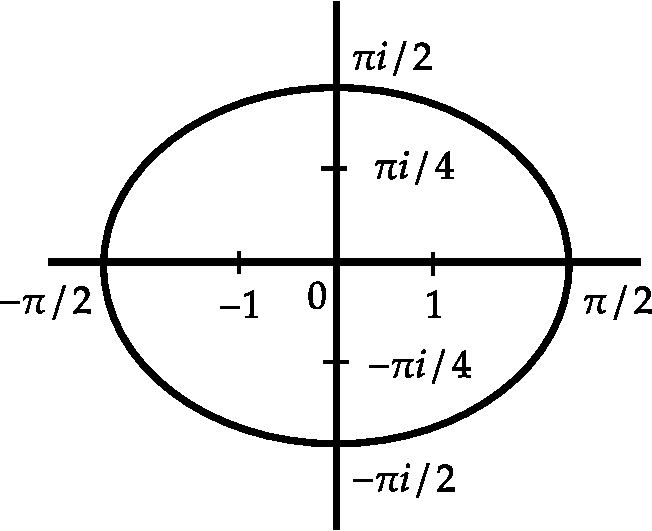
\includegraphics[height=4.5cm,width=5.5cm]{diagram-20211005(2)-crop}
		\end{figure}
		\begin{align*}
		&\oint_{C} \frac{d z}{z} \frac{\tanh 2 z}{\sin \pi z} d z\\
		z&=0,1,-1, \frac{\pi i}{4}, \frac{-\pi i}{4}\\
		f(z)&=\frac{2 z-\frac{1}{3}(2 z)^{3}+\frac{2}{15}(2 z)^{5} \ldots .}{z\left(\pi z-\frac{\pi^{3} z^{3}}{3 !}+\ldots\right)}\\
		\frac{2}{\pi z}&\left(1-\frac{1}{2} z^{2}+\ldots\right)\left(1-\frac{\pi^{2} z^{2}}{2 !}+\ldots\right)\\
		b_{1}&=\frac{2}{\pi}\\
		\text{As Re } z&=1, \frac{\tanh ^{2}}{-\pi}\text{ and }\operatorname{Re} z=-1, \frac{\tanh ^{2}}{-\pi}\\
		\operatorname{Re} z&=\frac{i \pi}{4}=-\frac{1}{\pi}\left(2 \operatorname{cosec} h \frac{\pi^{2}}{4}\right)\\
		\operatorname{Re} z&=\frac{-i \pi}{4}=-\frac{1}{\pi}\left(2 \operatorname{cosec} \mathrm{h} \frac{\pi^{2}}{4}\right)
		\intertext{$I=2 \pi i \Sigma R=4 i$ only when 0 lies inside, otherwise wrong question.}
		\end{align*}
		So the correct answer is \textbf{Option (B)}
	\end{answer}
	\item The integral $I=\int_{C} e^{z} d z$ is evaluated from the point $(-1,0)$ to $(1,0)$ along the contour $C$, which is an arc of the parabola $y=x^{2}-1$, as shown in the figure. The value of $I$ is
	{\exyear{NET/JRF(DEC-2018)}}
	\begin{figure}[H]
		\centering
		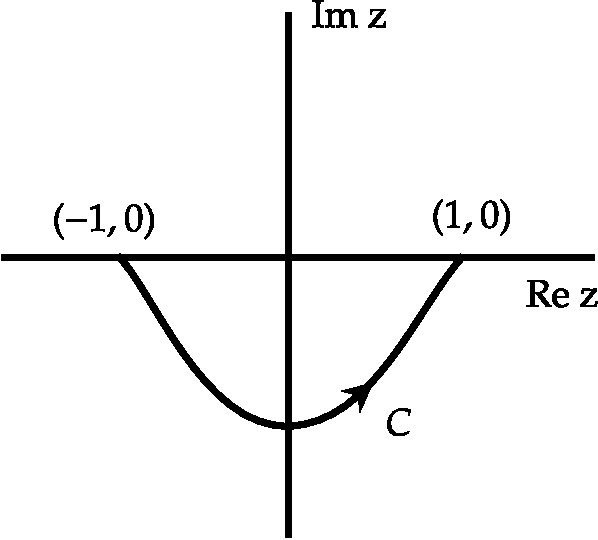
\includegraphics[height=4.5cm,width=5cm]{diagram-20211005(3)-crop}
	\end{figure}
	\begin{tasks}(4)
		\task[\textbf{A.}]  0
		\task[\textbf{B.}] $2 \sinh 1$
		\task[\textbf{C.}]  $e^{2 i} \sinh 1$
		\task[\textbf{D.}] $e+e^{-1}$
	\end{tasks}
	\begin{answer}
		\begin{align*}
		\int_{C} f(z) d z&=2 \pi i \Sigma R\\
		\int_{C} f(z) d z+\int_{1}^{-1} e^{x} d x&=0\\
		\int_{C} f(z) d z&=-\int_{1}^{-1} e^{x} d x=\int_{1}^{-1} e^{x} d x\\&=\frac{\left(e^{1}-e^{-1}\right)}{2} \cdot 2=2 \sinh 1
		\end{align*}
		So the correct answer is \textbf{Option (B)}
	\end{answer}
	\item The contour $C$ of the following integral
	$$
	\oint_{C} d z \frac{\sqrt{(z-1)(z-3)}}{\left(z^{2}-25\right)^{3}}
	$$
	in the complex $z$ plane is shown in the figure below.\\
	\begin{figure}[H]
		\centering
		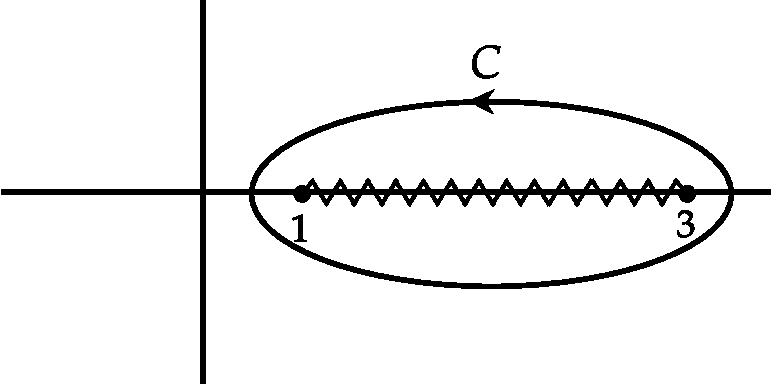
\includegraphics[height=3.5cm,width=6cm]{diagram-20211005(8)-crop}
	\end{figure}
	This integral is equivalent to an integral along the contours
	{\exyear{NET/JRF(DEC-2018)}}
	\begin{tasks}(2)
		\task[\textbf{A.}] \begin{figure}[H]
			\centering
			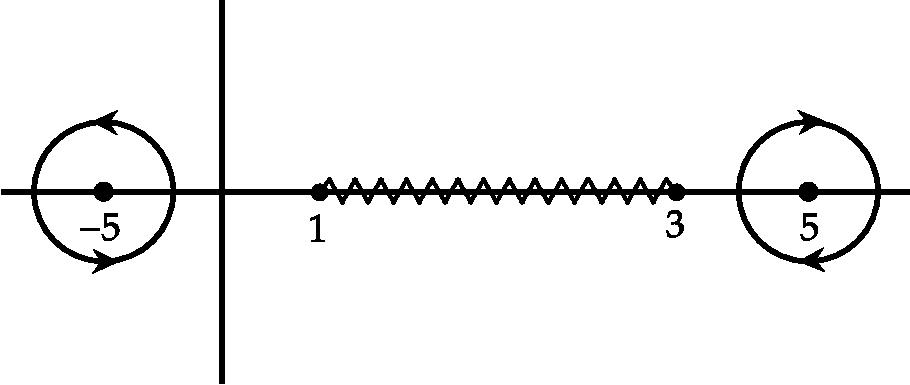
\includegraphics[height=3cm,width=6.5cm]{diagram-20211005(4)-crop}
		\end{figure}
		\task[\textbf{B.}] \begin{figure}[H]
			\centering
			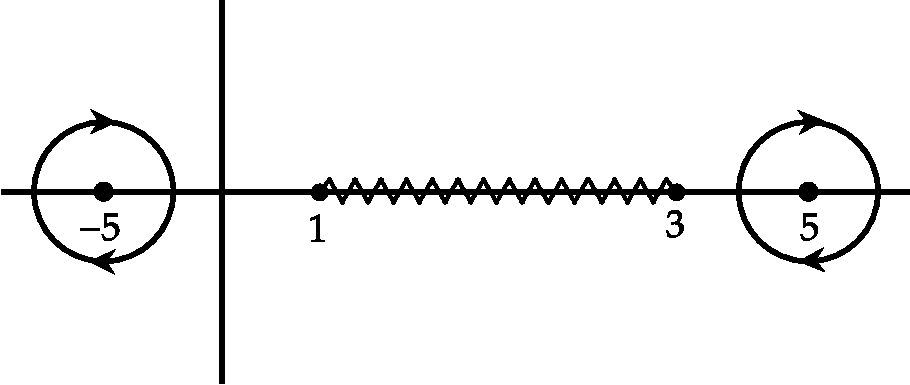
\includegraphics[height=3cm,width=6.5cm]{diagram-20211005(5)-crop}
		\end{figure}
		\task[\textbf{C.}] \begin{figure}[H]
			\centering
			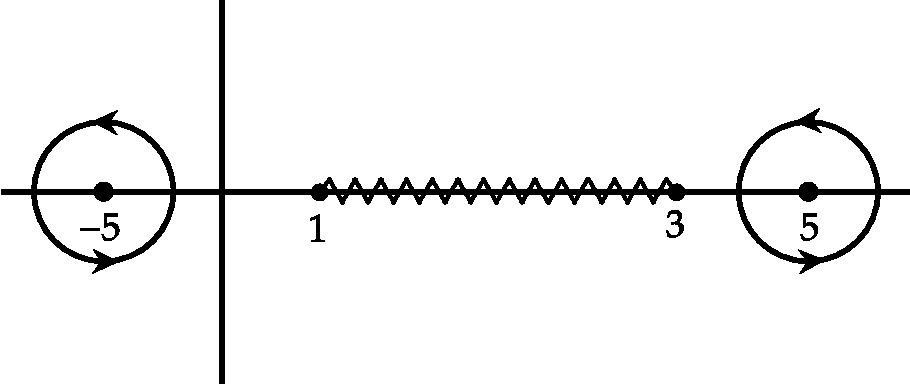
\includegraphics[height=3cm,width=6.5cm]{diagram-20211005(6)-crop}
		\end{figure}
		\task[\textbf{D.}] \begin{figure}[H]
			\centering
			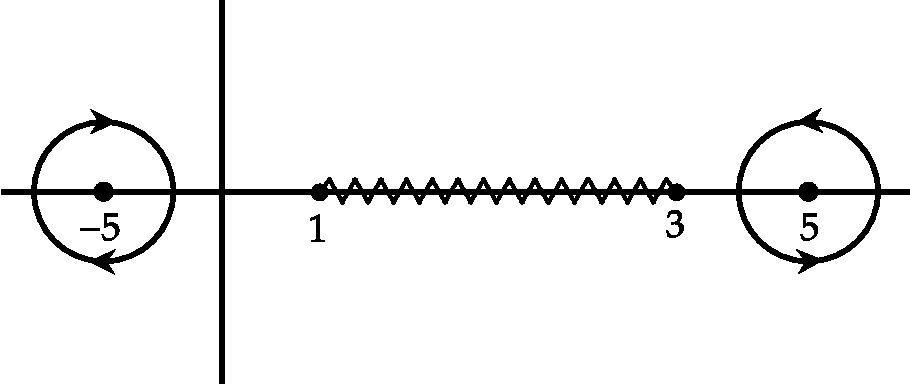
\includegraphics[height=3cm,width=6.5cm]{diagram-20211005(7)-crop}
		\end{figure}
	\end{tasks}
	\begin{answer}
		\begin{align*}
		\intertext{$z=1,3$ are branch points $\infty$ is not a branch point 1 branch cut 3}
		\end{align*}
		So the correct answer is \textbf{Option (C)}
	\end{answer}
	\item  Let $C$ be the circle of radius $\frac{\pi}{4}$ centered at $z=\frac{1}{4}$ in the complex $z$-plane that is traversed counter-clockwise. The value of the contour integral $\oint_{C} \frac{z^{2}}{\sin ^{2} 4 z} d z$ is
	{\exyear{NET/JRF(DEC-2019)}}
	\begin{tasks}(4)
		\task[\textbf{A.}] 0
		\task[\textbf{B.}] $\frac{i \pi^{2}}{4}$
		\task[\textbf{C.}] $\frac{i \pi^{2}}{16}$
		\task[\textbf{D.}] $\frac{i \pi}{4}$
	\end{tasks}
	\begin{answer}$\left. \right. $
		\begin{figure}[H]
			\centering
			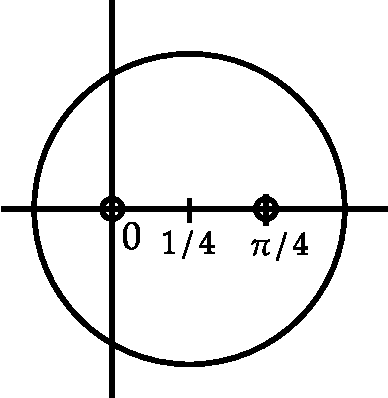
\includegraphics[height=3cm,width=3cm]{diagram-20211026(16)-crop}
		\end{figure}
		\begin{align*}
		f(z)&=\left(\frac{\pi}{\sin 4 z}\right)^{2}\\
		z_{0}&=0, \frac{\pi}{4}\text{ are poles}\\
		4 z&=n \pi, z=0, \frac{\pi}{4}
		\intertext{Others are outside the contour.}
		\text{Residue at }z&=0\text{ is }\left[\frac{\pi}{4 z-\frac{4^{3} z^{3}}{3 !}+\ldots}\right]^{2}\\
		&=\left[\frac{1}{4-\frac{4^{3} z^{2}}{3 !}+\ldots .}\right]^{2}\qquad \text{ No terms for } \frac{1}{z}, b_{1}=0\\
		&=\left[4-\frac{4^{3} z^{2}}{3 !}+\ldots .\right]^{-2}\\
		\text{Residue for }z&=\frac{\pi}{4}\\
		z-\frac{\pi}{4}&=t
		\intertext{$\sin (4 t+\pi)=-\sin 4 t \quad$ (But square so no effect)}
		&\left[\frac{t+\frac{\pi}{4}}{\sin 4\left(t+\frac{\pi}{4}\right)}\right]^{2}\\
		\left(\frac{t+\frac{\pi}{4}}{\sin 4 t}\right)^{2}&=\frac{t^{2}+\frac{\pi^{2}}{4}+2 t \cdot \frac{\pi}{4}}{\sin ^{2} 4 t}\\
		\frac{\pi}{2} \frac{t}{16 t^{2}[1-\ldots .]^{2}}&=\frac{\pi}{32 t}[1-\ldots .]^{-2} \text{(from first term)}\\
		b_{1}&=\frac{\pi}{32}\\
		\oint_{C} \frac{z^{2}}{\sin ^{2} 4 z} d z&=2 \pi i\left[0+\frac{\pi}{32}\right]=\frac{i \pi^{2}}{16}
		\end{align*}
		So the correct answer is \textbf{Option (C)}
	\end{answer}
	\item  A function of a complex variable $z$ is defined by the integral $f(z)=\oint_{\Gamma} \frac{w^{2}-2}{w-z} d w$, where $\Gamma$ is a circular contour of radius 3 , centred at origin, running counter-clockwise in the $w$ - plane. The value of the function at $z=(2-i)$ is
	{\exyear{NET/JRF(JUNE-2020)}}
	\begin{tasks}(4)
		\task[\textbf{A.}] 0
		\task[\textbf{B.}] $1-4 i$
		\task[\textbf{C.}]  $8 \pi+2 \pi \mathrm{i}$
		\task[\textbf{D.}] $-\frac{2}{\pi}-\frac{i}{2 \pi}$
	\end{tasks}
	\begin{answer}$\left. \right. $
		\begin{figure}[H]
			\centering
			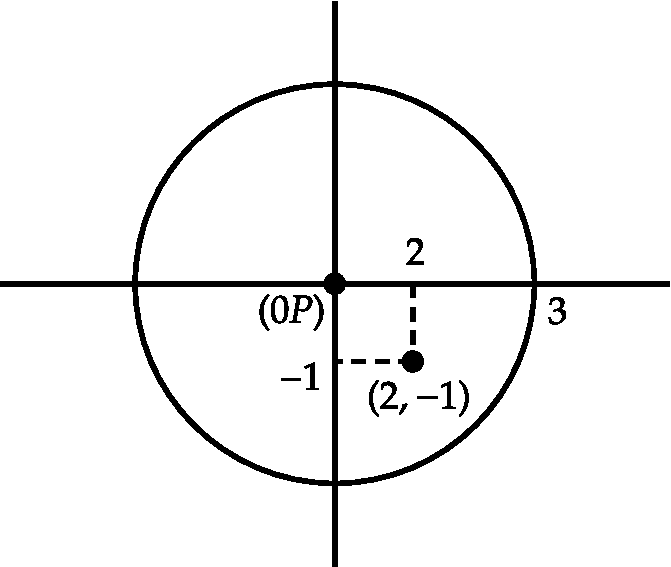
\includegraphics[height=4cm,width=4.6cm]{diagram-20211027-crop}
		\end{figure}
		\begin{align*}
		f(z)&=\oint_{\Gamma} \frac{w^{2}-2}{w-z} d w\\
		\omega&=z\text{ is a simple pole.}\\
		\text{Residue }\lim _{\omega \rightarrow z}(\omega-z) \frac{\left(\omega^{2}-2\right)}{(\omega-z)}&=(2-i)^{2}-2 \\&=4-1-4 i-2=(1-4 i)\\
		f(z)&=\oint_{\Gamma} \frac{w^{2}-2}{w-z} d w=2 \pi i(1-4 i)=2 \pi i+8 \pi
		\end{align*}
		So the correct answer is \textbf{Option (C)}
	\end{answer}
\end{enumerate}
\colorlet{ocre1}{ocre!70!}
\colorlet{ocrel}{ocre!30!}
\setlength\arrayrulewidth{1pt}
\begin{table}[H]
	\centering
	\arrayrulecolor{ocre}
	\begin{tabular}{|p{1.5cm}|p{1.5cm}||p{1.5cm}|p{1.5cm}|}
		\hline
		\multicolumn{4}{|c|}{\textbf{Answer key}}\\\hline\hline
		\rowcolor{ocrel}Q.No.&Answer&Q.No.&Answer\\\hline
		1&\textbf{C} &2&\textbf{B}\\\hline 
		3&\textbf{B} &4&\textbf{A} \\\hline
		5&\textbf{A} &6&\textbf{D} \\\hline
		7&\textbf{A}&8&\textbf{-}\\\hline
		9&\textbf{C}&10&\textbf{A}\\\hline
		11&\textbf{C} &12&\textbf{-}\\\hline
		13&\textbf{A}&14&\textbf{B}\\\hline
		15&\textbf{C}&16&\textbf{B}\\\hline
		17&\textbf{C} &18&\textbf{A}\\\hline
		19&\textbf{B}&20&\textbf{B}\\\hline
		21&\textbf{C}&22&\textbf{C}\\\hline
		23&\textbf{C}& &\\\hline
		
	\end{tabular}
\end{table}
\newpage
\begin{abox}
	Practise Set-2
\end{abox}
\begin{enumerate}[label=\color{ocre}\textbf{\arabic*.}]
	\item  The value of the integral $\oint_{C} \frac{e^{z} \sin (z)}{z^{2}} d z$, where the contour $C$ is the unit circle: $|z-2|=1$, is
	{\exyear{GATE 2010}}
	\begin{tasks}(4)
		\task[\textbf{A.}] $2 \pi i$
		\task[\textbf{B.}] $4 \pi i$
		\task[\textbf{C.}] $\pi i$
		\task[\textbf{D.}] 0
	\end{tasks}
	\item Which of the following statements is TRUE for the function $f(z)=\frac{z \sin z}{(z-\pi)^{2}}$ ?
	{\exyear{GATE 2011}}
	\begin{tasks}(1)
		\task[\textbf{A.}] $f(z)$ is analytic everywhere in the complex plane
		\task[\textbf{B.}] $f(z)$ has a zero at $z=\pi$
		\task[\textbf{C.}] $f(z)$ has a pole of order 2 at $z=\pi$
		\task[\textbf{D.}] $f(z)$ has a simple pole at $z=\pi$
	\end{tasks}
	\item For the function $f(z)=\frac{16 z}{(z+3)(z-1)^{2}}$, the residue at the pole $z=1$ is (your answer should be an integer)-------
	{\exyear{GATE 2013}}
	\item The value of the integral
	$$
	\oint_{C} \frac{z^{2}}{e^{z}+1} d z
	$$
	where $C$ is the circle $|z|=4$, is
	{\exyear{GATE 2014}}
	\begin{tasks}(4)
		\task[\textbf{A.}] $2 \pi i$
		\task[\textbf{B.}] $2 \pi^{2} i$
		\task[\textbf{C.}]  $4 \pi^{3} i$
		\task[\textbf{D.}] $4 \pi^{2} i$
	\end{tasks}
	\item Consider a complex function $f(z)=\frac{1}{z\left(z+\frac{1}{2}\right) \cos (z \pi)}$. Which one of the following statements is correct?
	{\exyear{GATE 2015}}
	\begin{tasks}(1)
		\task[\textbf{A.}] $f(z)$ has simple poles at $z=0$ and $z=-\frac{1}{2}$
		\task[\textbf{B.}] $f(z)$ has second order pole at $z=-\frac{1}{2}$
		\task[\textbf{C.}] $f(z)$ has infinite number of second order poles
		\task[\textbf{D.}] $f(z)$ has all simple poles
	\end{tasks}
	\item  Consider $w=f(z)=u(x, y)+i v(x, y)$ to be an analytic function in a domain $D$. Which one of the following options is NOT correct?
	{\exyear{GATE 2015}}
	\begin{tasks}(1)
		\task[\textbf{A.}] $u(x, y)$ satisfies Laplace equation in D
		\task[\textbf{B.}]  $v(x, y)$ satisfies Laplace equation in $D$
		\task[\textbf{C.}] $\int_{1}^{z_{2}} f(z) d z$ is dependent on the choice of the contour between $z_{1}$ and $z_{2}$ in $D$
		\task[\textbf{D.}]  $f(z)$ can be Taylor expended in $D$
	\end{tasks}
	\item A function $y(z)$ satisfies the ordinary differential equation $y^{\prime \prime}+\frac{1}{z} y^{\prime}-\frac{m^{2}}{z^{2}} y=0$, where\\
	$m=0,1,2,3, \ldots . .$ Consider the four statements P, Q, R, S as given below.\\
	$\mathrm{P}: z^{m}$ and $z^{-m}$ are linearly independent solutions for all values of $m$\\
	Q: $z^{m}$ and $z^{-m}$ are linearly independent solutions for all values of $m>0$\\
	$\mathrm{R}$ : $\ln z$ and 1 are linearly independent solutions for $m=0$\\
	S: $z^{m}$ and $\ln z$ are linearly independent solutions for all values of $m$\\
	The correct option for the combination of valid statements is
	{\exyear{GATE 2015}}
	\begin{tasks}(4)
		\task[\textbf{A.}] P, R and S only
		\task[\textbf{B.}]  P and R only
		\task[\textbf{C.}] $\mathrm{Q}$ and $\mathrm{R}$ only
		\task[\textbf{D.}] $\mathrm{R}$ and $\mathrm{S}$ only
	\end{tasks}
	\item  Which of the following is an analytic function of $z$ everywhere in the complex plane?
	{\exyear{GATE 2016}}
	\begin{tasks}(4)
		\task[\textbf{A.}] $z^{2}$
		\task[\textbf{B.}]  $\left(z^{*}\right)^{2}$
		\task[\textbf{C.}] $|z|^{2}$
		\task[\textbf{D.}] $\sqrt{z}$
	\end{tasks}
	\item The contour integral $\oint \frac{d z}{1+z^{2}}$ evaluated along a contour going from $-\infty$ to $+\infty$ along the
	real axis and closed in the lower half-plane circle is equal to............... (up to two decimal places).
	{\exyear{GATE 2017}}
	\item The imaginary part of an analytic complex function is $v(x, y)=2 x y+3 y .$ The real part of the function is zero at the origin. The value of the real part of the function at $1+i$ is ................. (up to two decimal places)
	{\exyear{GATE 2017}}
	\item The absolute value of the integral
	$$
	\int \frac{5 z^{3}+3 z^{2}}{z^{2}-4} d z
	$$
	over the circle $|z-1.5|=1$ in complex plane, is $\ldots$ (up to two decimal places).
	{\exyear{GATE 2018}}
	\item The pole of the function $f(z)=\cot z$ at $z=0$ is
	{\exyear{GATE 2019}}
	\begin{tasks}(2)
		\task[\textbf{A.}] A removable pole
		\task[\textbf{B.}] An essential singularity
		\task[\textbf{C.}]  A simple pole
		\task[\textbf{D.}] A second order pole
	\end{tasks}
	\item The value of the integral $\int_{-\infty}^{\infty} \frac{\cos (k x)}{x^{2}+a^{2}} d x$, where $k>0$ and $a>0$, is
	{\exyear{GATE 2019}}
	\begin{tasks}(4)
		\task[\textbf{A.}] $\frac{\pi}{a} e^{-k a}$
		\task[\textbf{B.}] $\frac{2 \pi}{a} e^{-k a}$
		\task[\textbf{C.}] $\frac{\pi}{2 a} e^{-k a}$
		\task[\textbf{D.}] $\frac{3 \pi}{2 a} e^{-k a}$
	\end{tasks}
\item The value of the integral $\int_{0}^{\infty} \frac{\ln x}{\left(x^{2}+1\right)^{2}} d x$ is
{\exyear{ JEST 2012}}
\begin{tasks}(2)
	\task[\textbf{a.}]0
	\task[\textbf{b.}]$\frac{-\pi}{4}$
	\task[\textbf{c.}] $\frac{-\pi}{2}$
	\task[\textbf{d.}] $\frac{\pi}{2}$
\end{tasks}
\item Compute $\lim _{z \rightarrow 0} \frac{\operatorname{Re}\left(z^{2}\right)+\operatorname{Im}\left(z^{2}\right)}{z^{2}}$
{\exyear{ JEST 2013}}
\begin{tasks}(2)
	\task[\textbf{a.}] The limit does not exist
	\task[\textbf{b.}]1
	\task[\textbf{c.}]$-i$
	\task[\textbf{d.}] $-1$
\end{tasks}
\item The value of limit
$$
\lim _{z \rightarrow i} \frac{z^{10}+1}{z^{6}+1}
$$
is equal to
{\exyear{ JEST 2014}}
\begin{tasks}(2)
	\task[\textbf{a.}]1
	\task[\textbf{b.}]0
	\task[\textbf{c.}] $\frac{-10}{3}$
	\task[\textbf{d.}] $\frac{5}{3}$
\end{tasks}
\item The value of integral
$$
I=\oint \frac{\sin z}{2 z-\pi} d z
$$
with $c$ a circle $|z|=2$, is
{\exyear{ JEST 2014}}
\begin{tasks}(2)
	\task[\textbf{a.}] 0
	\task[\textbf{b.}]$2 \pi i$
	\task[\textbf{c.}] $\pi i$
	\task[\textbf{d.}]  $-\pi i$
\end{tasks}
\item Given an analytic function $f(z)=\phi(x, y)+i \psi(x, y)$, where $\phi(x, y)=x^{2}+4 x-y^{2}+2 y$
If $C$ is a constant, which of the following relations is true?
{\exyear{ JEST 2015}}
\begin{tasks}(2)
	\task[\textbf{a.}]$\psi(x, y)=x^{2} y+4 y+C$
	\task[\textbf{b.}]$\psi(x, y)=2 x y-2 x+C$
	\task[\textbf{c.}]$\psi(x, y)=2 x y+4 y-2 x+C$
	\task[\textbf{d.}] $\psi(x, y)=x^{2} y-2 x+C$
\end{tasks}
\item Which one is the image of the complex domain $\{z \mid x y \geq 1, x+y>0\}$ under the mapping $f(z)=z^{2}$, if $z=x+i y ?$
{\exyear{ JEST 2017}}
\begin{tasks}(2)
	\task[\textbf{a.}] $\{z \mid x y \geq 1, x+y>0\}$
	\task[\textbf{b.}]$\{z \mid x \geq 2, x+y>0\}$
	\task[\textbf{c.}]$\{z \mid y \geq 2 \forall x\}$
	\task[\textbf{d.}] $\{z \mid y \geq 1 \forall x\}$
\end{tasks}
\item The integral $I=\int_{1}^{\infty} \frac{\sqrt{x-1}}{(1+x)^{2}} d x$ is
{\exyear{ JEST 2017}}
\begin{tasks}(2)
	\task[\textbf{a.}]$\frac{\pi}{\sqrt{2}}$
	\task[\textbf{b.}]$\frac{\pi}{2 \sqrt{2}}$
	\task[\textbf{c.}]$\frac{\sqrt{\pi}}{2}$
	\task[\textbf{d.}]$\sqrt{\frac{\pi}{2}}$
\end{tasks}
\item The integral
$$
\int_{-\infty}^{\infty} \frac{\cos x}{x^{2}+1} d x \text { is }
$$
{\exyear{ JEST 2018}}
\begin{tasks}(2)
	\task[\textbf{a.}]$\frac{\pi}{e}$
	\task[\textbf{b.}] $\pi e^{-2}$
	\task[\textbf{c.}]$\pi$
	\task[\textbf{d.}] zero
\end{tasks}
\item Consider the function $f(x, y)=|x|-i|y| .$ In which domain of the complex plane is this function analytic?
{\exyear{ JEST 2019}}
\begin{tasks}(2)
	\task[\textbf{a.}]First and second quadrants
	\task[\textbf{b.}]Second and third quadrants
	\task[\textbf{c.}]Second and fourth quadrants
	\task[\textbf{d.}]  Nowhere
\end{tasks}
\end{enumerate}
 \colorlet{ocre1}{ocre!70!}
\colorlet{ocrel}{ocre!30!}
\setlength\arrayrulewidth{1pt}
\begin{table}[H]
	\centering
	\arrayrulecolor{ocre}
	\begin{tabular}{|p{1.5cm}|p{1.7cm}||p{1.5cm}|p{1.5cm}|}
		\hline
		\multicolumn{4}{|c|}{\textbf{Answer key}}\\\hline\hline
		\rowcolor{ocrel}Q.No.&Answer&Q.No.&Answer\\\hline
		1&\textbf{D} &2&\textbf{C}\\\hline 
		3&\textbf{3(NAT)} &4&\textbf{C} \\\hline
		5&\textbf{A} &6&\textbf{C} \\\hline
		7&\textbf{C}&8&\textbf{A}\\\hline
		9&\textbf{$\pi$(NAT)}&10&\textbf{3(NAT)}\\\hline
		11&\textbf{81.64(NAT)} &12&\textbf{C}\\\hline
		13&\textbf{A}& 14&\textbf{B}\\\hline
		15&\textbf{A}&16 &\textbf{D}\\\hline
		17&\textbf{C}&18&\textbf{C}\\\hline
		19&\textbf{-} &20&\textbf{B}\\\hline
		21&\textbf{A}&22&\textbf{C}\\\hline
	\end{tabular}
\end{table}


